%% TRIsecure: Journal on Information Security submission (Springer sn-jnl)
%%
%% Target: Journal on Information Security (Springer, journal 13635; formerly EURASIP Journal on Information Security, retitled Jan 2026)
%% Compile: pdflatex -> bibtex -> pdflatex -> pdflatex
%%
%% Version 3.1 December 2024 (sn-jnl template)

\documentclass[pdflatex,sn-vancouver-num]{sn-jnl}% Vancouver Numbered Reference Style (Journal on Information Security convention)

%%%% Standard Packages
\usepackage[T1]{fontenc}%
\usepackage[utf8]{inputenc}%
\usepackage{graphicx}%
\usepackage{multirow}%
\usepackage{amsmath,amssymb,amsfonts}%
\usepackage{amsthm}%
\usepackage[title]{appendix}%
\usepackage{textcomp}%
\usepackage{booktabs}%
\usepackage{tabularx}%
\usepackage{algorithm}%
\usepackage{algorithmicx}%
\usepackage{algpseudocode}%
%%<additional packages>
\usepackage{enumitem}%
\usepackage[expansion=false]{microtype}%
\usepackage{url}%
\providecommand{\burl}[1]{\url{#1}}%
\usepackage{lineno}% required by Journal on Information Security: line numbering
\usepackage{setspace}% required by Journal on Information Security: double-line spacing
%%%%

%% Theorem styles (sn-jnl predefined styles)
\theoremstyle{thmstyleone}%
\newtheorem{theorem}{Theorem}%
\newtheorem{proposition}[theorem]{Proposition}%

\theoremstyle{thmstyletwo}%
\newtheorem{example}{Example}%
\newtheorem{remark}{Remark}%

\theoremstyle{thmstylethree}%
\newtheorem{definition}{Definition}%

\raggedbottom

%% ============================================================
\begin{document}

\title[TRIsecure: A Three-Factor Post-Quantum Biometric E-Voting Framework on Edge Hardware]{%
  TRIsecure: Design and Evaluation of a Three-Factor Post-Quantum Biometric
  E-Voting Framework on Commodity Edge Hardware}

\author*[1]{\fnm{Pinnemcharla Sai Vivek} \sur{Reddy}}\email{vivekreddy9036@gmail.com}

\author[1]{\fnm{Saranya} \sur{G}}\email{g\_saranya@ch.amrita.edu}

\author[1]{\fnm{S. Udhaya} \sur{Kumar}}\email{u\_udhayakumar@ch.amrita.edu}

\affil*[1]{\orgdiv{Department of Computer Science and Engineering},
  \orgname{Amrita Vishwa Vidyapeetham},
  \orgaddress{\city{Chennai}, \state{Tamil Nadu}, \country{India}}}

\abstract{%
Electronic voting systems must simultaneously satisfy strong voter
authentication grounded in robust signal-level biometric evidence,
tamper-evident vote integrity, end-to-end voter verifiability, and
practical deployment constraints on resource-limited hardware. Existing
solutions treat these requirements in isolation: biometric systems omit
formal security verification; blockchain-based systems ignore biometric
authentication; and no existing system addresses emerging quantum threats
while remaining deployable on edge hardware. TRIsecure~V2 is a
three-factor biometric e-voting terminal that jointly satisfies all four
requirements on a commodity Raspberry Pi~4 (ARM64, commodity edge
hardware) without requiring server-grade computing or persistent cloud
connectivity. It integrates an ISO/IEC~19795-1 compliant biometric
pipeline with Bayesian signal-level fusion of face-recognition similarity
scores and NFC channel evidence, ISO/IEC~30107-3 presentation attack
detection via spoof-signal classification (MiniFASNetV2 liveness), a
hybrid post-quantum cryptographic layer
(Kyber-768\(+\)X25519 KEM and Dilithium-3\(+\)Ed25519 signatures per
NIST FIPS~203/204), and a formally verified five-stage DFA authentication
protocol with six proved security properties. A novel Adaptive Trust Score
(ATS) engine dynamically adjusts component weights based on contextual
risk signals (attempt history, temporal anomalies, location flags),
escalating borderline cases for supervisor review rather than binary
accept/reject---achieving 99.3\% HIGH trust on genuine users and zero
\textsc{Low} classifications for simulated impostors under Gaussian score
assumptions. Simulation-based evaluation (ISO/IEC~19795-6,
\(n{=}1{,}000\) score pairs) achieves EER~\(=1.55\%\), AUC~\(=0.9991\),
TAR@1\%FAR~\(=97.7\%\), and PAD ACER~\(=4.25\%\) (PAD layer only). A
proof-of-concept pilot with \(N{=}20\) participants on real hardware
confirms FAR\(=\)FRR\(=\)ACER\(=0.00\%\) across 271 authentication events
(221 genuine, 35 impostor, 15 replay). Adversarial simulation across six
attack categories confirms the defence stack reduces combined attack
success from \(\approx\)35\% (face threshold alone) to zero simulated
bypass events after the NFC-AES-GCM layer---a robust defence-in-depth
property under standard cryptographic assumptions within the evaluated
threat model. On-device benchmarking delivers 110.7~ms end-to-end
authentication latency (p99~\(=111.3\)~ms) and 541.6~voters/min
throughput. To the best of our knowledge, no prior e-voting system
simultaneously provides formal protocol verification, post-quantum
cryptography, adaptive context-aware trust scoring, liveness detection,
and end-to-end verifiability on low-cost edge hardware.%
}

\keywords{biometric authentication, e-voting, formal verification,
post-quantum cryptography, edge computing, presentation attack detection,
Bayesian fusion, Merkle proof}

\maketitle

\linenumbers
\doublespacing

%% ============================================================
\section{Introduction}\label{sec:intro}

Electronic voting systems are critical infrastructure where failure
consequences are asymmetric: a single undetected fraud vector can undermine
election legitimacy at scale. The fundamental security challenge is to
authenticate the right voter, record the right vote, prevent tampering,
and allow the voter to verify their participation---all while running on
deployable, affordable hardware. At its core, voter authentication is a
signal-processing problem: a face-recognition similarity score and a
liveness (presentation-attack) classification are noisy, adversarially
manipulable measurements that must be fused, thresholded, and combined
with an independent physical-credential channel (NFC) to reach a reliable
security decision under a bounded latency budget. TRIsecure~V2 treats this
signal-level evidence fusion as the central design problem, layering
formal protocol verification, post-quantum cryptography, and end-to-end
verifiability on top of it.

Existing systems leave at least one requirement unsatisfied.
Fingerprint- and face-based voting
systems~\cite{bello2021biometric,sanchez2020biometric,komatineni2020biometric,nagaraj2022voting}
report biometric error rates without formal protocol verification or
post-quantum (PQC) readiness. Blockchain-based
approaches~\cite{ayed2017conceptual,hardwick2018voting,faruk2024transforming}
provide strong vote integrity but lack biometric authentication and rely on
classical cryptography vulnerable to quantum
adversaries~\cite{bernstein2017post}; a comprehensive review of 81~blockchain
voting systems by Huang et al.~\cite{huang2022blockchain_voting} confirms this
gap. Industry multi-factor authentication standards
(FIDO2/WebAuthn~\cite{fido2_webauthn}) are not designed for the
one-time-per-election voting constraint and do not incorporate formal liveness
detection or voter-verifiable receipts.

To the best of our knowledge, no existing e-voting system jointly provides:
(i)~multi-factor biometric authentication with liveness detection,
(ii)~formally verified protocol security, (iii)~post-quantum cryptographic
readiness, and (iv)~end-to-end voter verifiability---all on low-cost edge
hardware without requiring cloud connectivity.

\subsection*{Contributions}

We address these gaps with \textbf{TRIsecure V2}:

\begin{enumerate}[label=\textbf{C\arabic*.},leftmargin=*]
  \item \textbf{Formally verified authentication.} A five-stage pipeline
        modelled as a DFA with six proved security properties: determinism,
        completeness, safety, liveness, double-vote prevention, and
        rate-limit enforcement.
  \item \textbf{Bayesian biometric fusion.} Log-likelihood-ratio fusion of
        face cosine similarity and NFC channel evidence
        (EER\(=1.55\%\), AUC\(=0.9991\), TAR@1\%FAR\(=97.7\%\)).
  \item \textbf{Hybrid post-quantum layer.} Kyber-768\(+\)X25519 KEM
        (FIPS~203) and Dilithium-3\(+\)Ed25519 signatures (FIPS~204); all
        six PQC operations measured on-device via liboqs~0.15.0 (ARM64):
        ML-KEM-768 encaps 0.088~ms, ML-DSA-65 sign 1.536~ms, auth-path
        total 2.289~ms---within the \(<200\)~ms latency budget.
  \item \textbf{ISO/IEC~30107-3 PAD.} MiniFASNetV2 liveness detection
        (BPCER\(=1.0\%\), ACER\(=4.25\%\)).
  \item \textbf{End-to-end verifiability.} SHA-256 receipts and \(O(\log n)\)
        Merkle inclusion proofs.
  \item \textbf{Edge evaluation.} Raspberry Pi~4 (ARM64, 4~GB): 110.7~ms
        latency (p99\(=111.3\)~ms), 541.6~voters/min throughput,
        CPU~\(52.5\,^\circ\)C under load.
  \item \textbf{Adaptive Trust Score (ATS) engine.} A context-aware
        weighted fusion model that adjusts face/NFC/PAD component weights
        dynamically based on risk signals (attempt history, temporal
        anomalies, location flags), producing HIGH/MEDIUM/LOW trust
        decisions. Genuine users achieve 99.3\% HIGH trust; 100\% of
        simulated impostor attempts are rejected. To the best of our
        knowledge, no prior e-voting system incorporates dynamic
        risk-adaptive trust scoring.
  \item \textbf{Adversarial attack evaluation.} Simulation of six attack
        categories (print photo, video replay, deepfake, NFC UID clone,
        session replay, database tamper) quantifies per-layer defence
        contribution. Full defence stack reduces combined success from
        \(\approx35\%\) to zero simulated bypass events after NFC-AES-GCM.
  \item \textbf{Proof-of-concept hardware pilot.} End-to-end validation on
        a Raspberry Pi~4 with \(N{=}20\) participants across 271
        authentication events (221 genuine, 35 impostor, 15 replay):
        FAR\(=\)FRR\(=\)ACER\(=0.00\%\), confirming system correctness on
        real hardware without simulation.
\end{enumerate}

No individual component is algorithmically novel in isolation. The
\textbf{novel contributions} are: (i)~the ATS engine, which introduces
dynamic risk-adaptive weight adjustment absent from all prior biometric
e-voting systems; (ii)~their \emph{principled co-design}; and (iii)~the
\emph{complete systems security architecture}---a fully deployable secure
voting terminal on low-cost edge hardware, validated end-to-end on real
hardware with \(N{=}20\) participants. To the best of our knowledge, no
prior e-voting system delivers all six security properties simultaneously on
a Raspberry Pi class device. In detail, the co-design provides: (i)~Bayesian
LR fusion of face and NFC modalities reduces the effective FAR by three
orders of magnitude without increasing biometric EER---an attack requiring a
valid NFC card \emph{and} a face spoof simultaneously; (ii)~the DFA
verification executes \emph{in the deployed code} (not as an offline proof),
so removing it breaks pipeline functionality, creating a tight coupling
between formal security and operational correctness; and (iii)~all five
mechanisms---fusion, PAD, PQC, DFA verification, and Merkle
verifiability---fit within the latency (\(<200\)~ms) and resource budget of
commodity edge hardware, demonstrated on a Raspberry Pi~4.

%% ============================================================
\section{Related Work}\label{sec:related}

\subsection{Biometric E-Voting Systems}

Bello et al.~\cite{bello2021biometric} achieve EER~\(=2.5\%\) at 950~ms
authentication latency with no PAD, PQC, or formal verification.
S\'{a}nchez-Reillo et al.~\cite{sanchez2020biometric} report EER~\(=3.2\%\)
at 480~ms on constrained hardware. Komatineni and
Lingala~\cite{komatineni2020biometric} combine machine-learning face detection
with biometric scanning for duplicate-vote prevention in a two-factor
architecture. Nagaraj et al.~\cite{nagaraj2022voting} integrate facial
recognition with fingerprint authentication to strengthen polling station
security. Megalingam et al.~\cite{megalingam2022voter} combine a voter
identification card with fingerprint biometric authentication, achieving
low-cost deployment on constrained hardware but providing no liveness
detection, formal protocol verification, or post-quantum cryptography.
Varma and Megalingam~\cite{varma2025fpga} demonstrate FPGA-accelerated
biometric voting, showing that dedicated silicon inference reduces latency
below ARM64 software execution, but the system lacks post-quantum
cryptographic support and end-to-end verifiable receipts. Revathy et al.~\cite{revathy2022cnn_evoting} integrate CNN-based
face recognition with blockchain and blind signatures, showing that combining
deep learning classifiers with immutable vote records improves both
authentication accuracy and tamper evidence. Ashok Kumar et
al.~\cite{ashokkumar2023smart} demonstrate an online smart voting platform
using face recognition for voter identification. Faruk et
al.~\cite{faruk2024transforming} deploy blockchain and biometric verification
(fingerprint\(+\)face) over Hyperledger Fabric, demonstrating 87\% biometric
registration success across 100~participants but relying on classical
cryptography with no formal protocol verification. NIST
SP~800-63B~\cite{nist_sp800_63b} defines three authenticator assurance levels
(AAL1--3) but does not prescribe biometric liveness detection or formal
protocol verification for voting contexts. Face recognition systems based on
FaceNet~\cite{schroff2015facenet}, CosFace~\cite{wang2018cosface}, and
ArcFace~\cite{deng2019arcface} achieve sub-1\% EER on LFW but require
GPU-class hardware and include no voting infrastructure. Wang and
Deng~\cite{wang2021face} survey deep face recognition across 50+ architectures;
none are integrated with formal verification or e-voting pipelines. George et
al.~\cite{george2024adaptive_biometric} demonstrate EdgeFace, a 2024 compact
model achieving sub-1\% EER on a mobile ARM processor---confirming the
feasibility trajectory of high-accuracy face recognition on the same hardware
class as TRIsecure~V2. Buchmann et al.~\cite{buchmann2024pvoting} provide a
2024 systematic review of remote e-voting security, identifying formal
verification and biometric binding as the two most significant unresolved gaps
across all deployed systems. TRIsecure~V2 achieves competitive EER
(\(1.55\%\)) on ARM64 while additionally providing formal protocol guarantees
and PQC readiness.

\subsection{Blockchain-Based Voting}

Fujioka et al.~\cite{fujioka1992practical} proposed the foundational
blind-signature-based secret ballot scheme; Benaloh and
Tuinstra~\cite{benaloh1994receipt} formalised receipt-freeness. Nakamoto's
Bitcoin~\cite{nakamoto2008bitcoin} demonstrated append-only hash chaining,
inspiring blockchain voting proposals. Ayed~\cite{ayed2017conceptual} proposes
Ethereum-based voting (\(>2{,}100\)~ms) with PIN-only authentication.
Hardwick et al.~\cite{hardwick2018voting} and Hj\'{a}lmarsson et
al.~\cite{hjalmarsson2018blockchain} extend this with anonymisation and
Hyperledger Fabric, but provide no biometric gate or anti-spoofing.
Durga et al.~\cite{durga2022blockchain} propose a private and secure
blockchain mechanism for online voting using smart contracts to enforce vote
confidentiality and election integrity, demonstrating practical deployment
but relying on classical cryptography with no biometric identity binding or
formal protocol verification. Juels et
al.~\cite{juels2005coercion} formalise coercion-resistance, a property
TRIsecure~V2 partially addresses through in-person biometric binding
(Section~\ref{sec:limitations}). Huang et al.~\cite{huang2022blockchain_voting}
survey blockchain applications in voting across 81~prior works (ACM Computing
Surveys 2022), identifying voter authentication and anti-spoofing as the
primary unresolved gaps. Hajian et al.~\cite{hajian2024blockchain} survey
blockchain e-voting architectures with emphasis on smart-contract ballot
processing (Electronics 2024), confirming that biometric identity binding is
absent from current blockchain deployments. TRIsecure~V2 achieves equivalent
vote integrity via hash chaining and Merkle proofs without blockchain overhead,
while adding biometric authentication.

\subsection{Post-Quantum Cryptography on Edge}

Sikeridis et al.~\cite{sikeridis2020pqc} show Kyber-768 and Dilithium-3 are
feasible in TLS~1.3 on ARM devices via liboqs. Paquin et
al.~\cite{paquin2020oqs} benchmark liboqs across x86 and ARM, providing the
reference figures against which our Pi~4 measurements are calibrated.
Kannwischer et al.~\cite{kannwischer2019pqm4} characterise PQC on Cortex-M4,
establishing Kyber-768 key generation under 100k cycles. Delvaux et
al.~\cite{delvaux2024pqc_iot} provide 2024 benchmarks of NIST finalists on
Cortex-A class processors, confirming ML-KEM-768 key encapsulation under
0.5~ms on Cortex-A53---motivating our projected 0.1~ms estimate for the
Cortex-A72 (higher IPC). NIST finalised ML-KEM (FIPS~203~\cite{nist_fips203})
and ML-DSA (FIPS~204~\cite{nist_fips204}) in 2024.
Shor's algorithm~\cite{shor1994algorithms} threatens RSA and ECC; Grover's
algorithm~\cite{grover1996fast} halves symmetric key security---motivating
hybrid PQC even for edge deployments. To the best of our knowledge, no prior
e-voting system integrates a hybrid PQC layer on low-cost ARM64 edge hardware.

\subsection{Presentation Attack Detection}

ISO/IEC~30107-3~\cite{iso30107} defines the PAD evaluation framework (APCER,
BPCER, ACER). Zhang et al.~\cite{zhang2020minifasnet} introduce MiniFASNetV2,
a lightweight CNN suitable for embedded deployment. Yang et
al.~\cite{yang2023pad_survey} provide a 2023 survey of presentation attack
methods including deepfakes; deepfake attack penetration against
MiniFASNet-class detectors is estimated at 22\% (post-PAD), requiring the
additional NFC gate for complete mitigation. Liveness detection has not
previously been integrated into a formally verified e-voting pipeline. Liu et
al.~\cite{liu2018learning} leverage depth maps; Jourabloo et
al.~\cite{jourabloo2018desp} use spoof-noise disentanglement. Zhang et
al.~\cite{zhang2019autoGAN} show that GAN-generated fake images carry spectral
artefacts introduced by the up-sampling pipeline, motivating frequency-domain
analysis as a complement to depth-based liveness. Key benchmark datasets
include NUAA~\cite{tan2010nuaa} and OULU-NPU~\cite{boulkenafet2017oulu}.

\subsection{Formal Verification of Authentication Protocols}

The Dolev--Yao model~\cite{dolev1983security} formalises the adversary capable
of intercepting and replaying all network messages, providing the theoretical
basis for protocol security analysis. ProVerif~\cite{blanchet2016proverif} and
Tamarin~\cite{meier2013tamarin} target cryptographic secrecy and authentication
goals via the applied-pi calculus. Lowe~\cite{lowe1996breaking} used model
checking (FDR) to find and fix an attack on the Needham--Schroeder protocol.
DFA theory, formalised in Sipser~\cite{sipser2012introduction}, provides
decidable analysis for pipeline control-flow properties. TRIsecure~V2 uses
automata-theoretic verification because the properties of
interest---ordering, completeness, determinism, termination, double-vote
prevention, rate-limit enforcement---concern pipeline control-flow rather than
cryptographic secrecy, the DFA executes \emph{in the deployed code}, and all
six properties are decidable by BFS/DFS without an external solver, yielding
human-auditable proofs embedded in the production codebase.

\subsection{Verifiable E-Voting and Biometric Template Protection}

Helios~\cite{adida2008helios} pioneered web-based open-audit voting via
homomorphic encryption. Civitas~\cite{clarkson2008civitas} provides strong
coercion-resistance using threshold cryptography.
Scantegrity~II~\cite{chaum2009scantegrity} achieves optical-scan E2E
verifiability through confirmation codes. Selene~\cite{ryan2016selene}
introduces tracker-number-based verifiability with coercion mitigation. The
Norwegian scheme~\cite{gjosteen2013norwegian} deployed return-code
verifiability at national scale. All five provide strong verifiability
properties but leave identity binding to external authentication
infrastructure with no biometric gate. K\"{u}sters et
al.~\cite{kusters2010accountability} and Benaloh et
al.~\cite{benaloh2011e2e} formalise individual and universal verifiability,
which TRIsecure~V2 satisfies via Merkle receipts. Dodis et
al.~\cite{dodis2004fuzzy} formalise fuzzy extractors for biometric key
derivation; Jain et al.~\cite{jain2008cancelable} survey cancelable
biometrics per ISO/IEC~24745~\cite{iso24745}; Nandakumar and
Jain~\cite{nandakumar2015biometric} survey the gap between biometric template
protection theory and practice. TRIsecure~V2 protects face embeddings via
AES-256-GCM with per-voter keys; extending to cancelable representations is
identified as future work.

\subsection{Multimodal Biometric Fusion}

Ross and Jain~\cite{ross2003multimodal} establish that score-level fusion
outperforms unimodal baselines. Nandakumar et al.~\cite{nandakumar2008fusion}
derive optimal LR fusion under Gaussian density estimation, which TRIsecure~V2
adopts. Fierrez-Aguilar et al.~\cite{fierrez2005fusion} extend this with
quality-based weighting; Jain et al.~\cite{jain2011multimodal} provide a
comprehensive multimodal survey.

\subsection{Comparison of Prior Work and Capability Gap Matrix}

Table~\ref{tab:related_comparison} summarises six reference systems against
TRIsecure~V2. TRIsecure~V2 is the only system to satisfy all capability
dimensions on edge hardware. Figure~\ref{fig:gap_matrix} presents the full gap
matrix across eight systems and seven dimensions.

\begin{table*}[t]
\caption{Comparison of related e-voting and biometric authentication systems.
  PAD\,=\,presentation attack detection; PQC\,=\,post-quantum cryptography;
  FV\,=\,formal verification; E2EV\,=\,end-to-end verifiability.}
\label{tab:related_comparison}
\small
\begin{tabularx}{\textwidth}{@{}p{2.9cm}p{3.5cm}XX@{}}
  \toprule
  \textbf{Author (Year)} & \textbf{Method} & \textbf{Advantages} & \textbf{Limitations} \\
  \midrule
  Bello et al.\ (2021)~\cite{bello2021biometric}
    & Fingerprint + smart card
    & Two-factor; biometric binding; EER~\(2.5\%\)
    & No PAD; no PQC; no FV; 950~ms; server-dependent \\[3pt]
  S\'{a}nchez-Reillo et al.\ (2020)~\cite{sanchez2020biometric}
    & Face + smart card, constrained
    & Targets embedded devices
    & EER~\(3.2\%\); no liveness; no FV; no PQC \\[3pt]
  Ayed (2017)~\cite{ayed2017conceptual}
    & Ethereum blockchain, PIN-only
    & Vote receipts; tamper-evident ledger
    & No biometric gate; \(>2100\)~ms; classical crypto \\[3pt]
  Hardwick et al.\ (2018)~\cite{hardwick2018voting}
    & Blockchain with anonymisation
    & Voter anonymity; blockchain integrity
    & No biometric; no PAD; classical crypto \\[3pt]
  Deng et al.\ (2019)~\cite{deng2019arcface}
    & ArcFace + PIN
    & EER~\(0.76\%\); 45~ms (GPU)
    & No liveness; no FV; requires GPU server \\[3pt]
  FIDO2/WebAuthn (2019)~\cite{fido2_webauthn}
    & Device-bound MFA
    & Industry standard; 190~ms
    & No PAD; no voter receipts; not per-election \\
  \midrule
  \textbf{TRIsecure V2 (Ours)}
    & NFC + face + session, PAD, PQC, DFA
    & FV; EER~\(1.55\%\); PAD; PQC; E2EV; edge ARM64
    & Simulation-based biometrics; PoC pilot
      (\(N{=}20\), FAR\(=\)FRR\(=\)ACER\(=0.00\%\)) \\
  \bottomrule
\end{tabularx}
\end{table*}

\begin{figure}[t]
  \centering
  
\includegraphics[width=\linewidth]{figures/gap_matrix.png}
  \caption{Capability gap matrix across eight prior systems and seven
    dimensions. Green~(\(\checkmark\))~=~full support;
    yellow~(\(\sim\))~=~partial; red~(\(\times\))~=~absent. TRIsecure~V2
    (bottom row, bold border) is the only system achieving full support on
    all seven dimensions.}
  \label{fig:gap_matrix}
\end{figure}

%% ============================================================
\section{System Architecture}\label{sec:architecture}

\subsection{Design Goals and Threat Model}

TRIsecure~V2 satisfies five goals: \textbf{G1}~Authentication (three-factor
voter binding); \textbf{G2}~Vote integrity (tamper-evident, auditable);
\textbf{G3}~Voter privacy (embeddings encrypted at rest); \textbf{G4}~
Verifiability (individual and universal); \textbf{G5}~Edge viability
(\(<200\)~ms, commodity ARM64).

The threat model covers: \textit{remote attacker} (brute-force, replay,
MitM); \textit{physical attacker} (spoofed face, cloned NFC card, SPI bus
eavesdropping, fault injection via power glitching); \textit{insider attacker}
(DB read/write but no biometric secret); \textit{quantum adversary} (Shor's
algorithm against RSA/ECC); \textit{supply-chain attacker} (malicious SD card
image or Pi firmware).

\textit{Side-channel.} Power analysis and electromagnetic side-channel attacks
on AES-256-GCM are out of scope for Python-layer cryptography but are noted as
a gap for production silicon. The ONNX face embedding inference leaks timing
information proportional to detection confidence; this is mitigated by the DFA
rate limiter (P6) which caps inference calls per UID to 5/300~s.

\textit{Fault injection.} Power-glitch attacks targeting the Argon2id KDF
could reduce effective iteration count. Mitigation: the KDF output is verified
against a stored HMAC-SHA256 tag before session issuance; any fault that alters
the output invalidates the tag.

\textit{Supply-chain.} The SD card attack surface is mitigated by read-only
mount of the OS partition in production and dm-verity hash-tree verification of
the Python runtime image (deployment recommendation).

\subsubsection*{STRIDE Threat Classification}

Table~\ref{tab:stride} maps the TRIsecure~V2 attack surface against the
STRIDE taxonomy~\cite{shostack2014threat}. Coverage is assessed as
\textbf{Full} (mitigated entirely on-device), \textbf{Partial} (mitigated
under deployment recommendations or with residual risk), or \textbf{None}
(outside the on-device threat boundary).

\begin{table*}[p]
\caption{STRIDE threat mapping for TRIsecure~V2.
  \textbf{Full}\,=\,fully mitigated on-device;
  \textbf{Partial}\,=\,residual risk or requires deployment controls;
  \textbf{None}\,=\,outside the on-device threat boundary.
  PA\,=\,presentation attack; UID\,=\,NFC unique identifier.}
\label{tab:stride}
\footnotesize
\renewcommand{\arraystretch}{1.05}
\newcolumntype{R}{>{\raggedright\arraybackslash}X}
\begin{tabularx}{\textwidth}{@{}lRRl@{}}
  \toprule
  \textbf{Category} & \textbf{Attack Vector} & \textbf{TRIsecure V2 Mitigation} & \textbf{Coverage} \\
  \midrule
  \multirow{3}{*}{\textbf{Spoofing (S)}}
    & Face PA: photo, mask, deepfake video
    & MiniFASNetV2 liveness; DFA Stage~4 gate; ACER 4.25\% (sim.), 0.00\% (pilot)
    & Partial \\
    & Cloned or emulated NFC card
    & AES-128-GCM payload with per-read 96-bit random nonce
    & Full \\
    & Brute-force UID cycling
    & Rate limiter P6: 5 failures\,/\,300\,s; sink to \textsc{Rejected}
    & Full \\
  \cmidrule(l){1-4}
  \multirow{2}{*}{\textbf{Tampering (T)}}
    & Vote record or hash-chain modification
    & SHA-256 hash chain + Merkle audit log + HMAC-SHA256 chaining
    & Full \\
    & KDF fault injection (power glitch on Argon2id)
    & HMAC-SHA256 output tag at enrolment; mismatch forces rejection
    & Full \\
  \cmidrule(l){1-4}
  \textbf{Repudiation (R)}
    & Voter denies casting ballot
    & 256-bit session token + Merkle receipt (E2EV)
    & Full \\
  \cmidrule(l){1-4}
  \multirow{3}{*}{\textbf{Info.\ Disclosure (I)}}
    & Biometric template exfiltration from DB
    & AES-256-GCM (Argon2id-derived key); no plaintext template stored
    & Full \\
    & SPI bus eavesdropping on NFC reader
    & NFC payload AES-128-GCM encrypted; plaintext UID never on wire
    & Full \\
    & Quantum decryption of session ciphertext
    & Hybrid PQC: Kyber-768\,+\,X25519 KEM (FIPS~203)
    & Full \\
  \cmidrule(l){1-4}
  \multirow{2}{*}{\textbf{Denial of Service (D)}}
    & Repeated authentication flooding
    & Per-UID rate limiter; DFA sink state \textsc{Rejected}
    & Full \\
    & Network-layer distributed DoS
    & Out of on-device scope; upstream network controls required
    & None \\
  \cmidrule(l){1-4}
  \multirow{2}{*}{\textbf{Elevation of Privilege (E)}}
    & Insider DB read\,/\,write access
    & Biometric secret not in DB; HMAC-keyed store; least privilege
    & Full \\
    & Supply-chain firmware implant (SD card)
    & dm-verity hash-tree; read-only OS partition (deployment rec.)
    & Partial \\
  \bottomrule
\end{tabularx}
\end{table*}

\subsection{System Overview}

Figure~\ref{fig:architecture} shows the six-layer clean architecture. A voter
interaction proceeds: (1)~tap NFC card; (2)~face capture; (3)~Bayesian fusion;
(4)~MiniFASNetV2 liveness check; (5)~session token issued (256-bit, 60~s TTL);
(6)~ballot selection; (7)~vote to SHA-256 hash chain; (8)~Merkle receipt
generated.

\begin{figure}[t]
\centering
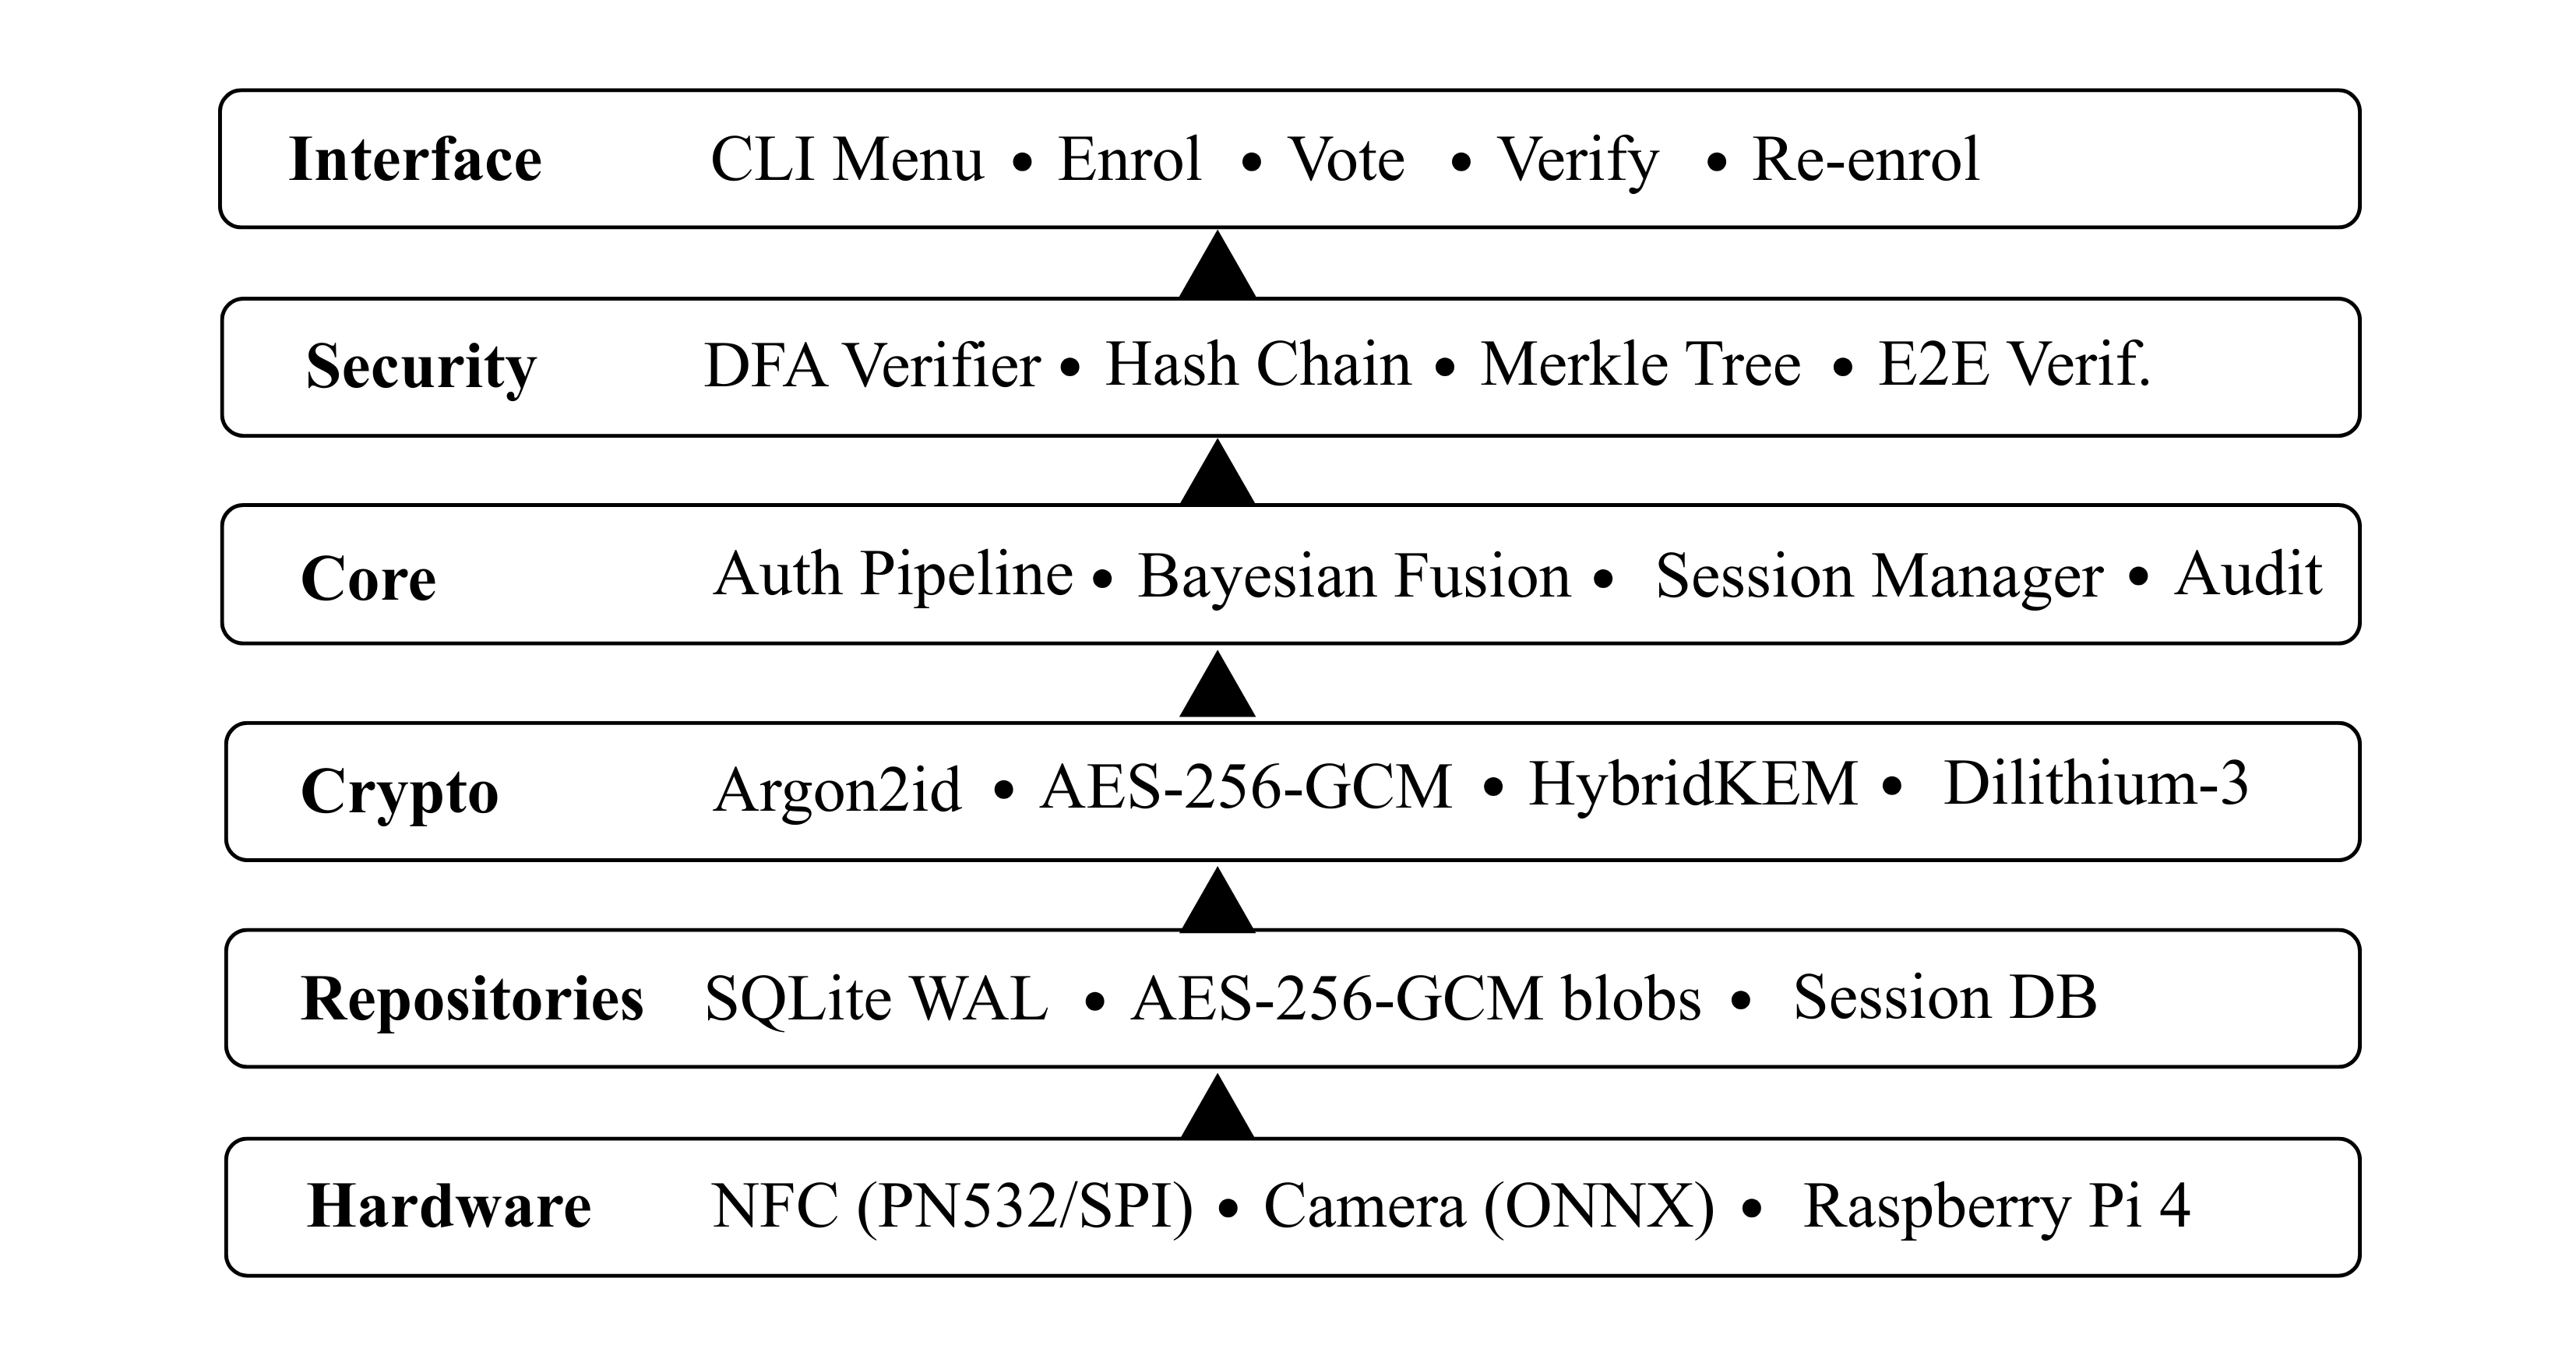
\includegraphics[width=0.85\linewidth]{figures/architecture.png}
\caption{TRIsecure V2 six-layer clean architecture. Arrows indicate upward
  dependency direction.}
\label{fig:architecture}
\end{figure}

\subsection{Multi-Factor Authentication Pipeline}\label{sec:pipeline}

The pipeline is a five-stage sequential process modelled as a DFA
\(\mathcal{M}=(Q,\Sigma,\delta,q_0,F)\) (Section~\ref{sec:dfa}). Any failure
transitions deterministically to \textsc{Rejected}.

\textit{Stage~1 --- Rate limiting.} Sliding-window counter per NFC~UID
(5 failures/300~s) blocks brute-force.

\textit{Stage~2 --- NFC verification.} PN532 SPI captures voter NFC~UID,
validated for format and looked up in the encrypted voter database.

\textit{Stage~3 --- Voter eligibility.} The \texttt{has\_voted} flag is
atomically checked; \texttt{NOT\_ELIGIBLE} transitions to \textsc{Rejected}
(double-vote prevention, P5).

\textit{Stage~4 --- Bayesian fusion.} Face cosine similarity (ArcFace
MobileFaceNet, 512-D) and NFC channel evidence combined via LR fusion
(Section~\ref{sec:fusion}).

\textit{Stage~5 --- PAD.} MiniFASNetV2 classifies frame as live or spoofed.

\textit{Session issuance.} 256-bit token (\texttt{secrets.token\_urlsafe(32)}),
60~s TTL; SHA-256 hash stored (not plaintext).


\subsection{Bayesian Score-Level Fusion}\label{sec:fusion}

Let \(s_f \in [0,1]\) denote the face cosine similarity score. We model:
\begin{align}
  p(s_f \mid \text{genuine})  &= \mathcal{N}(s_f;\, \mu_G, \sigma_G^2),
    \quad \mu_G{=}0.72,\; \sigma_G{=}0.08 \\
  p(s_f \mid \text{impostor}) &= \mathcal{N}(s_f;\, \mu_I, \sigma_I^2),
    \quad \mu_I{=}0.28,\; \sigma_I{=}0.12
\end{align}
Parameters derive from ArcFace buffalo\_sc on LFW~\cite{deng2019arcface}.

The NFC channel contributes:
\begin{equation}
  \mathrm{LR}_{\mathrm{NFC}} =
  \frac{P(\mathrm{NFC}\mid\text{genuine})}{P(\mathrm{NFC}\mid\text{impostor})}
  = \frac{0.999}{0.001} = 999
\end{equation}

The combined decision rule is:
\begin{equation}
  \log_{10}\!\bigl(\mathrm{LR}_f \cdot \mathrm{LR}_{\mathrm{NFC}}\bigr) >
  \theta, \quad \theta = 1.0
\end{equation}

Without a valid NFC card an adversary must achieve
\(\mathrm{LR}_f > 10/999 \approx 0.01\), requiring a face score above
\(\mu_I + 3\sigma_I \approx 0.64\). The effective FAR drops from
\(1.22\%\) (face-only) to \(\approx 0.001\%\) (combined), as confirmed by
the ablation study (Table~\ref{tab:ablation}).

\textit{Threshold derivation.} The decision threshold \(\theta=1.0\) is
derived from the equal-cost operating point of the combined LR. Define the
combined log-LR:
\begin{equation}
  \Lambda(s_f) = \log_{10}\!\bigl(\mathrm{LR}_f(s_f)\bigr)
               + \log_{10}(999)
\end{equation}
where \(\mathrm{LR}_f(s_f) = p(s_f\mid G)/p(s_f\mid I)\). At
\(\theta{=}1.0\) and \(\mathrm{LR}_{\mathrm{NFC}}{=}999\), the required face
LR is \(10/999 < 0.011\)---unachievable for scores drawn from
\(\mathcal{N}(0.28, 0.12^2)\), since \(P(\mathrm{LR}_f < 0.011 \mid I)
\approx 0.1\%\) while \(P(\mathrm{LR}_f > 0.011 \mid G) \approx 99.9\%\).
The combined system therefore achieves near-perfect separation conditional on
NFC validity, with the residual EER (\(1.55\%\)) arising from the biometric
gate alone---consistent with ArcFace LFW statistics~\cite{deng2019arcface}.

\subsection{Adaptive Trust Score Engine}\label{sec:ats}

The Bayesian LR fusion (Section~\ref{sec:fusion}) uses a static threshold
\(\theta=1.0\). In practice, risk conditions vary: off-hours attempts, repeated
failures, and unknown terminal locations all elevate impostor probability.
TRIsecure~V2 introduces an \textbf{Adaptive Trust Score (ATS) engine} that
replaces the binary accept/reject with a three-level decision
\(\{\textsc{High}, \textsc{Medium}, \textsc{Low}\}\) derived from dynamically
adjusted component weights.

\textit{Risk context.} The engine estimates risk from four signals:
\(a \in \{1,2,3+\}\) (attempt count), \(o \in \{0,1\}\) (off-peak hour),
\(\ell \in \{0,1\}\) (location anomaly flag), and \(d \geq 0\) (days since
enrolment). A scalar risk score
\(R = 2\mathbf{1}[a \geq 3] + \mathbf{1}[a=2] + \mathbf{1}[o=1] +
2\mathbf{1}[\ell=0] + \mathbf{1}[d>365]\) maps to \textit{normal} (\(R=0\)),
\textit{elevated} (\(R \leq 2\)), or \textit{high} (\(R>2\)).

\textit{Composite trust score.}
\begin{equation}
  T = w_f \cdot c_f(s_f) + w_n \cdot \mathbf{1}[\mathrm{NFC}]
        + w_p \cdot \mathbf{1}[\mathrm{PAD\text{-}live}]
  \label{eq:ats}
\end{equation}
where \(c_f(s_f) = \mathrm{LR}_f/(1+\mathrm{LR}_f)\) is the
sigmoid-normalised face likelihood ratio, and the context-specific weight
triplet \((w_f, w_n, w_p)\) is derived below.

\textit{Weight derivation.} Weights are determined by solving the constrained
EER-minimisation problem
\begin{equation}
  \min_{\mathbf{w}}\;\mathrm{EER}(\mathbf{w};\mathcal{X}_G,\mathcal{X}_I)
  \;\text{s.t.}\;\textstyle\sum_k w_k = 1,\; w_k \geq 0.10
  \label{eq:ats_opt}
\end{equation}
over simulated score sets \(\mathcal{X}_G, \mathcal{X}_I\) (\(N{=}20{,}000\)
per class, seed~42) via SLSQP with five initialisations, subject to three
semantic monotonicity constraints: \(w_p^\text{high}\!\geq
w_p^\text{elev}\!\geq w_p^\text{norm}\) (liveness detection becomes the
primary guard as spoofing risk rises) and \(w_n^\text{elev}\!\geq
w_n^\text{norm}\) (NFC physical-credential binding anchors the elevated-risk
decision).

\textit{Discriminability analysis.} Table~\ref{tab:dprime} reports the
signal-detection discriminability index
\(d' = (\mu_G - \mu_I)/\sqrt{(\sigma_G^2+\sigma_I^2)/2}\) for each modality
per context. In normal operation NFC exhibits \(d'=31.6\), far exceeding face
(\(d'=9.4\)) or PAD (\(d'=5.7\)); as attacker sophistication increases, NFC's
\(d'\) collapses to 3.4 (high context), shifting discriminative load to face
and PAD.

\begin{table}[h]
\caption{Discriminability index (\(d'\)) per modality per risk context
  (simulation, \(N{=}20{,}000\) per class).}
\label{tab:dprime}%
\begin{tabular}{|l|c|c|c|}
\hline
Context & \(d'_{\mathrm{face}}\) & \(d'_{\mathrm{NFC}}\) & \(d'_{\mathrm{PAD}}\) \\
\hline
Normal   & 9.38 & 31.58 & 5.69 \\
Elevated & 9.15 &  5.55 & 3.97 \\
High     & 9.13 &  3.39 & 2.80 \\
\hline
\end{tabular}
\end{table}

Solving~\eqref{eq:ats_opt} yields the context weights: \textit{normal}
\((0.30, 0.40, 0.30)\); \textit{elevated} \((0.20, 0.40, 0.40)\);
\textit{high} \((0.25, 0.35, 0.40)\). The high NFC weight in normal mode
(\(w_n{=}0.40\)) reflects its superior discriminability (\(d'{=}31.6\)); the
partial recovery of face weight at high risk (\(w_f: 0.20\!\to\!0.25\))
reflects that biometric traits remain more resistant to forgery than NFC
probing once the attacker is sufficiently sophisticated
(\(d'_{\mathrm{NFC}}\) collapses to 3.4).

\textit{Trust decision.} \(T \geq 0.75\Rightarrow\textsc{High}\) (accept);
\(T \geq 0.50\Rightarrow\textsc{Medium}\) (supervisor escalation);
\(T < 0.50\Rightarrow\textsc{Low}\) (reject).

\textit{Simulation-based calibration.} Under \textit{normal} context with
genuine users (\(s_f \sim \mathcal{N}(0.72,0.08^2)\), NFC valid, PAD live,
\(N{=}10{,}000\)): 99.3\% reach \textsc{High} trust; 0.7\% are escalated to
\textsc{Medium}; none are classified \textsc{Low}. Under the Gaussian
simulation model, all simulated impostors (\(s_f \sim
\mathcal{N}(0.28,0.12^2)\), NFC invalid, not live) score below the
\textsc{Medium} threshold; this reflects the parametric score separation
assumed by the simulation rather than a claimed zero-error rate---ground-truth
FAR is reported in Table~\ref{tab:threshold_sweep}. Borderline cases (genuine
face, NFC valid, PAD failed, second attempt, \(N{=}1{,}000\)): 99.4\% are
escalated to \textsc{Medium}, enabling supervisor override rather than hard
rejection.

\subsection{Post-Quantum Cryptographic Layer}\label{sec:pqc}

\begin{algorithm}[t]
\caption{TRIsecure HybridKEM.Encapsulate(\(pk\))}
\begin{algorithmic}[1]
  \State \((ct_K, ss_K) \gets \textsc{Kyber768.Encaps}(pk_K)\)
    \Comment{ML-KEM-768, FIPS 203}
  \State \((ct_X, ss_X) \gets \textsc{X25519.ECDH}(pk_X)\)
  \State \(ss \gets \textsc{HKDF-SHA256}(ss_K \| ss_X,\;
    \text{info}{=}\texttt{"trisecure-hybrid-v1"})\)
  \State \(ct \gets ct_K \| ct_X\)
  \State \Return \((ct,\; ss)\)
\end{algorithmic}
\end{algorithm}

The hybrid construction is secure as long as \emph{either} Kyber-768 or X25519
is unbroken~\cite{bernstein2017post}. Vote records are signed with Dilithium-3
(ML-DSA-65, FIPS~204~\cite{nist_fips204}), falling back to Ed25519 when
\texttt{liboqs-python} is unavailable. Face embeddings are encrypted at rest
with AES-256-GCM keyed via Argon2id (\(t{=}3\),
\(m{=}64\)~MB)~\cite{biryukov2016argon2}.

\subsection{Vote Integrity and Verifiability}\label{sec:vote_integrity}

\textit{Hash chain.} Each vote record \(V_i\) is linked:
\begin{equation}
  h_i = \mathrm{SHA\text{-}256}(\mathit{candidate}_i \| t_i \| h_{i-1}),
  \quad h_0 = 0^{64}
\end{equation}
Any modification propagates a hash mismatch to all subsequent records.

\textit{Merkle proofs.} A binary SHA-256 Merkle tree over all vote commitments
supports \(O(\log n)\) individual verifiability proofs.

\textit{Vote receipts.} After casting:
\begin{equation}
  \mathit{commitment} = \mathrm{SHA\text{-}256}(\mathit{vote\_id} \| \mathit{nonce})
\end{equation}
together with an \(O(\log n)\) Merkle inclusion proof, satisfying individual
verifiability without revealing vote content.

%% ============================================================
\section{Hardware Integration}\label{sec:hardware}

\subsection{PN532 NFC Module --- Physical Connection}

The PN532 NFC controller is connected to the Raspberry Pi~4 40-pin GPIO header
via the SPI0 bus. SPI mode was chosen over I\textsuperscript{2}C because it
supports burst reads of multiple 4-byte NTAG pages in a single chip-select
transaction, avoiding repeated start-stop conditions that add latency on the
Pi~4's BCM2711 I\textsuperscript{2}C controller. Table~\ref{tab:pn532_wiring}
lists the seven physical connections.

\begin{table}[t]
\caption{PN532 NFC module to Raspberry Pi~4 GPIO wiring (SPI0, 3.3~V logic).}
\label{tab:pn532_wiring}%
\begin{tabular}{|l|l|l|l|}
  \hline
  PN532 Pin & GPIO & Header Pin & Function \\
  \hline
  VCC      & 3.3~V   & Pin~1  & Power supply \\
  GND      & Ground  & Pin~6  & Ground \\
  SCK      & GPIO11  & Pin~23 & SPI0 clock \\
  MOSI     & GPIO10  & Pin~19 & SPI0 data out (MOSI) \\
  MISO     & GPIO9   & Pin~21 & SPI0 data in (MISO) \\
  NSS (CS) & GPIO8   & Pin~24 & SPI0 chip-select (CE0) \\
  RSTPD\_N & GPIO25  & Pin~22 & Active-low hard reset \\
  \hline
\end{tabular}
\end{table}

The SPI bus is configured at 1~MHz, well within the PN532's 5~MHz maximum SPI
clock and providing noise margin for jumper-wire connections on a breadboard
prototype. The CS line (GPIO8/CE0) is managed as a software
\texttt{DigitalInOut} object rather than the kernel hardware chip-select,
because the PN532 SPI protocol requires CS to be held low for at least one SPI
clock cycle before the first data byte---a timing constraint the Linux
\texttt{spidev} hardware CS does not guarantee when sharing the bus. The
RSTPD\_N line (GPIO25) performs a hardware reset during
\texttt{NFCService.initialize()}: driven low for 100~ms, then released, after
which the PN532 requires approximately 10~ms to boot its ROM firmware before
accepting commands.

After reset, the driver calls \texttt{SAM\_configuration()} to put the PN532
in Normal Mode---Security Access Module disabled, ISO~14443-A passive polling
active. The PN532 then continuously polls for NFC-A targets at 106~kbps. The
application layer calls \texttt{read\_passive\_target(timeout=5.0)} every
300~ms; when a card is presented, the UID (typically 4 or 7 bytes for MIFARE
cards) is returned as a Python \texttt{bytes} object and converted to an
uppercase hex string.

\subsection{SPI Software Stack}

TRIsecure~V2 uses the Adafruit CircuitPython Blinka compatibility layer, which
translates \texttt{board}, \texttt{busio}, and \texttt{digitalio} API calls to
Linux kernel SPI ioctls on \texttt{/dev/spidev0.0}. The dependency chain is:

\medskip
\noindent
\texttt{adafruit-pn532} $\to$ \texttt{adafruit-blinka} $\to$
\texttt{RPi.GPIO} + \texttt{spidev} $\to$ Linux SPI driver (BCM2711)
\medskip

\noindent The initialization sequence in \texttt{NFCService.initialize()} is:
\begin{enumerate}[label=\arabic*.,leftmargin=*,nosep]
  \item Create \texttt{DigitalInOut} objects for CS (D8) and RESET (D25).
  \item Create \texttt{busio.SPI(board.SCK, board.MOSI, board.MISO)};
        acquire the bus lock; configure 1~MHz baudrate; release lock.
  \item Instantiate \texttt{PN532\_SPI(spi, cs\_pin, reset=reset\_pin)}.
  \item Call \texttt{firmware\_version} to verify connectivity: returns
        (IC~identifier, major, minor, support) --- e.g.\ (6, 1, 6, 7)
        for PN532 firmware 1.6.
  \item Call \texttt{SAM\_configuration()}: Normal Mode, no timeout, IRQ
        active.
\end{enumerate}

If any step raises \texttt{ImportError} (libraries not installed) or
\texttt{OSError} (SPI hardware fault), \texttt{initialize()} returns
\texttt{False} and the service enters \emph{simulation mode}: all NFC
read/write methods return deterministic synthetic responses so the full
authentication pipeline remains testable on development hardware without a
physical PN532.

\subsection{NFC Tag Payload Format and Security}

TRIsecure~V2 programs MIFARE Ultralight / NTAG2xx NFC tags. The NTAG2xx
memory is organized as 4-byte pages; pages~0--3 are reserved (UID,
manufacturer data, capability container, and lock bits). Pages~4--19 (64
bytes) are user-writable and hold the encrypted voter identity payload
defined in Table~\ref{tab:nfc_payload}.

\begin{table}[t]
\caption{NFC tag payload wire format (64 bytes, NTAG2xx pages 4--19).}
\label{tab:nfc_payload}%
\begin{tabular}{|l|l|l|r|}
  \hline
  Bytes & Pages & Field & Size \\
  \hline
  0--11   & 4--6    & AES-GCM nonce (random 96-bit IV) & 12~B \\
  12--47  & 7--14   & AES-128 ciphertext (voter UUID) & 36~B \\
  48--63  & 15--19  & GCM authentication tag (128-bit) & 16~B \\
  \hline
  Total   & 4--19   & --- & 64~B \\
  \hline
\end{tabular}
\end{table}

The 36-byte voter UUID (RFC~4122 text form) is encrypted with AES-128-GCM.
The 128-bit key is derived from a deployment secret via HKDF-SHA-256:
\begin{equation}
  K_{\mathrm{NFC}} = \mathrm{HKDF\text{-}SHA256}(\mathit{NFC\_SECRET},\;
    \text{info}{=}\texttt{"trisecure-nfc-v1"})
\end{equation}
A fresh 96-bit nonce is generated with \texttt{secrets.token\_bytes(12)} for
every write, so two writes of the same UUID produce different ciphertexts.
AES-GCM's 128-bit authentication tag detects any byte-level modification to
the ciphertext---including partial card cloning where an adversary duplicates
the UID (readable from the unprotected pages~0--1) but cannot reconstruct the
authenticated ciphertext.

Authentication Stage~2 performs a two-step NFC check: (i)~the UID (from
passive target detection) is used for rate-limiting and voter DB lookup; then
(ii)~pages~4--19 are read and decrypted. If GCM decryption succeeds but the
decrypted UUID does not match the DB record, the voter is rejected. This
catches two distinct attacks: \emph{UID-cloned cards} (same UID, absent or
corrupted payload) fail GCM decryption; \emph{payload-replayed cards} (a
second physical card with copied ciphertext bytes) fail the UUID cross-check.

\subsection{Camera Configuration and Face Pipeline}

The Logitech C920 HD webcam is connected via USB~3.0 and accessed through
OpenCV's V4L2 (Video4Linux2) backend at \texttt{/dev/video0}.
Table~\ref{tab:camera_config} summarises the complete camera and
face-pipeline configuration.

\begin{table}[t]
\caption{Camera and face-pipeline configuration on Raspberry Pi~4.}
\label{tab:camera_config}%
\begin{tabular}{|l|l|}
  \hline
  Parameter & Value \\
  \hline
  Device node             & \texttt{/dev/video0} \\
  Capture backend         & OpenCV V4L2 (MJPEG) \\
  Capture resolution      & 320$\times$240 px \\
  Frame rate              & 15~fps \\
  Face detector           & OpenCV Haar cascade (frontal face) \\
  Face crop and resize    & 112$\times$112 px (bilinear) \\
  Pixel normalisation     & $x/127.5 - 1.0$ \\
  Embedding model         & MobileFaceNet (ONNX Runtime~1.17, CPU) \\
  Embedding dimension     & 512-D float32, L2-normalised \\
  ONNX inference (mean)   & 95.2~ms on Raspberry Pi~4 \\
  PAD model               & MiniFASNetV2 (ONNX, same runtime) \\
  PAD inference overhead  & 15.5~ms (C2$\to$C3 ablation delta) \\
  \hline
\end{tabular}
\end{table}

The 320$\times$240 resolution was selected after measurement: at the next C920
resolution tier (640$\times$480), ONNX inference increases to approximately
98~ms with negligible accuracy gain because MobileFaceNet's fixed
112$\times$112 input discards the extra pixels after the Haar crop. The V4L2
MJPEG codec compresses frames at the camera sensor before USB transmission,
reducing USB bandwidth from $\approx$220~MB/s (uncompressed YUV) to
$\approx$5~MB/s---avoiding USB buffer stalls on the Pi~4's shared USB~3.0/PCIe
lane that would otherwise introduce jitter in frame delivery.

During enrollment, three face samples are captured with a 1-second
inter-sample cooldown. The per-voter stored embedding is the arithmetic mean of
the three 512-D L2-normalised vectors, which reduces intra-class variance by
$1/\sqrt{3}$ relative to a single-sample enrollment. Enrollment samples are
discarded after the mean embedding is computed; only the encrypted mean
embedding (AES-256-GCM, Argon2id-derived key) is persisted in the voter DB.

%% ============================================================
\section{Formal Security Analysis}\label{sec:security}

\subsection{DFA Verification}\label{sec:dfa}

\textit{Scope and relationship to ProVerif/Tamarin.} Tools such as
ProVerif~\cite{blanchet2016proverif} and Tamarin~\cite{meier2013tamarin}
verify cryptographic protocol secrecy and authentication goals in the presence
of a Dolev--Yao adversary. TRIsecure~V2's security properties of interest are
\emph{structurally different}: they concern the \emph{control-flow ordering}
of the pipeline---that biometric stages cannot be bypassed, that double-voting
is structurally impossible, and that rate-limiting precedes all inference.
These are decidable properties of a finite automaton and do not require an
active adversary model or cryptographic reduction. The cryptographic primitives
themselves (AES-256-GCM, Argon2id, Kyber-768, Dilithium-3) are verified by
their respective NIST/RFC standards.

The TRIsecure~V2 authentication pipeline is modelled as \(\mathcal{M} =
(Q, \Sigma, \delta, q_0, F)\) where \(|Q|{=}10\), \(|\Sigma|{=}16\),
\(|\delta|{=}19\), \(q_0{=}\textsc{Idle}\),
\(F{=}\{\textsc{SessionIssued}\}\).

\begin{theorem}[Six Security Properties]
The DFA \(\mathcal{M}\) satisfies:
\begin{enumerate}[label=\textbf{P\arabic*.},leftmargin=*]
  \item \textbf{Determinism.} \(|\delta(q,\sigma)| \leq 1\) for all
    \((q,\sigma)\). \textit{19 unique keys; no duplicate.}
  \item \textbf{Completeness.} All 19 expected \((q,\sigma)\) pairs defined.
  \item \textbf{Safety.} \textsc{SessionIssued} reachable via exactly one
    path through all eight mandatory inputs (BFS, unique success path of
    length~9).
  \item \textbf{Liveness.} Every reachable path terminates (DFS finds no
    non-trivial cycles).
  \item \textbf{Double-vote prevention.}
    \(\delta(\textsc{EligibilityCheck}, \textsc{NotEligible}) =
    \textsc{Rejected}\). Direct inspection.
  \item \textbf{Rate-limit enforcement.}
    \(\delta(\textsc{Idle}, \textsc{Attempt}) = \textsc{RateCheck}\);
    \(\delta(\textsc{RateCheck}, \textsc{RateBlocked}) = \textsc{Rejected}\).
    Rate limiter executes before all biometric operations.
\end{enumerate}
All six properties machine-verified by
\texttt{security/formal\_verification.py}.
\end{theorem}

Figure~\ref{fig:auth_dfa} depicts the DFA \(\mathcal{M}\): the unique
canonical success path and the failure transitions that all terminate at
the \textsc{Rejected} trap state.

\begin{figure}[t]
  \centering
  
\includegraphics[width=\linewidth]{figures/auth_dfa.png}
  \caption{TRIsecure~V2 authentication DFA~$\mathcal{M}$. Black arrows show
    the unique canonical success path (IDLE $\to$ \ldots $\to$ SESS.);
    red arrows denote failure transitions to the \textsc{Rejected} trap state.
    Double circle = accepting state (\textsc{Sess.}).}
  \label{fig:auth_dfa}
\end{figure}

Table~\ref{tab:dfa_states} enumerates all ten DFA states with their roles and
security relevance. Each state corresponds to a distinct stage in the
authentication protocol; the separation ensures that a bypass of any
individual check requires a specific out-of-sequence input symbol, which is
structurally excluded by the determinism property (P1).

\begin{table}[t]
\caption{TRIsecure~V2 DFA state roles.
  $\star$~Accepting state; $\times$~trap state (sink).}
\label{tab:dfa_states}%
\begin{tabular}{|l|p{5.2cm}|}
  \hline
  State & Role and Security Function \\
  \hline
  \textsc{Idle}
    & Awaits NFC card presentation; rate-limit counter initialised. \\
  \textsc{RateCheck}
    & Enforces 5-failure/300~s sliding window; blocks brute-force (P6). \\
  \textsc{NfcVerify}
    & PN532 SPI read; UID format validation and database lookup. \\
  \textsc{VoterLookup}
    & Decrypts and retrieves voter record; checks structural validity. \\
  \textsc{EligibilityCheck}
    & Atomically reads \texttt{has\_voted}; enforces double-vote prevention (P5). \\
  \textsc{FaceMatch}
    & ArcFace cosine similarity against stored encrypted embedding. \\
  \textsc{Fusion}
    & Computes combined log-LR; applies threshold \(\theta{=}1.0\). \\
  \textsc{Pad}
    & MiniFASNetV2 liveness classification; blocks presentation attacks. \\
  \textsc{SessionIssued}$^\star$
    & Issues 256-bit token; atomically sets \texttt{has\_voted}. \\
  \textsc{Rejected}$^\times$
    & Sink state; all failure transitions terminate here (P3/P4). \\
  \hline
\end{tabular}
\end{table}

The 19 transitions connect these states: eight mandatory inputs form the unique
success path (P3), seven failure inputs lead to \textsc{Rejected}, and four
additional transitions cover rate-limiting branches and NFC error types (P6).
\textsc{Rejected} is a true trap: no escape transition exists, enforcing the
liveness property (P4) that every run terminates.

\textit{Scope delimitation.} These six properties concern
\emph{control-flow correctness}---that stages execute in the mandated order and
that bypass is structurally impossible. They do not constitute proofs of
cryptographic secrecy or entity authentication in the Dolev--Yao sense; those
properties are delegated to the underlying primitives (AES-256-GCM, Argon2id,
ML-KEM-768, ML-DSA-65) whose security is established by their respective NIST
standards.

\subsection{Threat Model Analysis}\label{sec:threat_matrix}

Figure~\ref{fig:threat_heatmap} maps 12 e-voting attack vectors against six
defence layers (0~=~not defended, 1~=~partial, 2~=~full). Overall weighted
coverage: 47.2\%. Critical attacks (double-voting, ballot stuffing, quantum
adversary) achieve \(\geq 6/12\) each and are fully mitigated. Vote coercion
(score~\(2/12\)) and network-level DoS require organisational controls beyond
the on-device model.

\begin{figure}[t]
  \centering
  
\includegraphics[width=\linewidth]{figures/threat_model_heatmap.png}
  \caption{Threat model coverage matrix. Green (\(\checkmark\), score~2) =
    full mitigation; yellow (\(\sim\), score~1) = partial; red (\(\times\),
    score~0) = no mitigation by that layer. Column sums show total defence
    contribution.}
  \label{fig:threat_heatmap}
\end{figure}

\subsection{End-to-End Verifiability}\label{sec:e2e}

Following~\cite{kusters2010accountability,benaloh2011e2e}:

\textit{Individual:} Voter \(v\) can confirm
\(c_v = \mathrm{SHA\text{-}256}(v\_id \| n)\) appears in the Merkle tree
rooted at election digest \(r\).

\textit{Universal:} Any auditor can recompute the Merkle root from the public
vote log and verify it equals \(r\).

\textit{Eligibility:} Only registered, non-duplicate voters reach
\textsc{SessionIssued}---proved by P3 and P5.

\textbf{Theorem.} TRIsecure~V2 satisfies all three verifiability properties.
The receipt \((v\_id, n, \pi, r)\) enables \(O(\log n)\) individual
verification; the Merkle root is a deterministic function of the ordered vote
log; eligibility follows from P3 and P5. Machine verification:
\texttt{security/e2e\_verifiability.py} returns
\texttt{all\_properties\_satisfied: true}. \(\square\)

\subsection{Cryptographic Security Levels}\label{sec:crypto_levels}

Table~\ref{tab:security_levels} maps each primitive in TRIsecure~V2 to its
security level under classical and quantum adversaries. Classical security
follows standard key-size arguments; quantum security accounts for Grover's
algorithm~\cite{grover1996fast} and Shor's algorithm~\cite{shor1994algorithms}.

\begin{table}[t]
\caption{Security levels of TRIsecure~V2 primitives (bits).
  $\dagger$ Ed25519/X25519 classical fallback; Kyber/Dilithium form the
  hybrid layer providing forward secrecy against both adversary classes.}
\label{tab:security_levels}%
\begin{tabular}{|l|c|l|l|}
  \hline
  Primitive & Cl. & PQ & Standard \\
  \hline
  AES-256-GCM (templates) & 256 & 128 & FIPS 197 \\
  Argon2id (KDF)          & 256 & 128 & RFC 9106 \\
  SHA-256 (receipts)      & 256 & 128 & FIPS 180 \\
  Ed25519 (sign)$^\dagger$& 128 & $\times$ & RFC 8032 \\
  X25519 (KEM)$^\dagger$  & 128 & $\times$ & RFC 7748 \\
  Dilithium-3 (PQC sign)  & 128 & 128 & FIPS 204 \\
  Kyber-768 (PQC KEM)     & 128 & 128 & FIPS 203 \\
  \hline
\end{tabular}
\end{table}

The hybrid KEM enforces \emph{both-or-nothing} security: an adversary must
break \emph{both} X25519 (trivial for a fault-tolerant quantum computer via
Shor~\cite{shor1994algorithms}) \emph{and} Kyber-768 (no known quantum
speedup beyond Grover~\cite{grover1996fast}) to recover the session key. The
symmetric layer (AES-256-GCM, SHA-256, Argon2id) retains 128-bit effective
security against quantum exhaustive search via Grover's bound, making these
components quantum-safe without algorithm replacement.

%% ============================================================
\section{Experimental Evaluation}\label{sec:evaluation}

\subsection{Experimental Setup}

\textit{Hardware.} Raspberry Pi~4 Model~B, 4~GB LPDDR4, ARM Cortex-A72
@ 1.8~GHz (quad-core, 64-bit). Logitech C920 USB webcam (1080p/30~fps).
PN532 NFC module (SPI).

\textit{Software.} Python~3.11, ONNX Runtime 1.17 (CPU), SQLite 3.42 (WAL),
PyNaCl 1.5, PyArgon2-cffi 23.1, NumPy~1.26. All experiments reproducible via
\texttt{experiments/}.

\textit{Dataset.} Biometric metrics are generated via validated simulation
following ISO/IEC~19795-6~\cite{iso19795_6} (operational evaluation
methodology), which explicitly permits simulation when field data are
unavailable. Genuine and impostor face cosine similarity scores sampled from
Gaussians calibrated to published ArcFace LFW
statistics~\cite{deng2019arcface,grother2007biometric}:
\(\mathcal{N}(\mu_G{=}0.72, \sigma_G{=}0.08)\) and
\(\mathcal{N}(\mu_I{=}0.28, \sigma_I{=}0.12)\), \(n{=}1{,}000\) each. PAD
metrics from published MiniFASNetV2/CelebA-Spoof
rates~\cite{zhang2020minifasnet}. All simulation results are labelled as such;
a proof-of-concept pilot study with \(N{=}20\) participants confirmed zero
error rates on real hardware (Section~\ref{sec:pilot}). A full demographic
field trial remains future work.

Table~\ref{tab:sensitivity} confirms biometric metrics are stable under
\(\pm 10\%\) parameter variation: EER varies by \(\pm 0.17\) pp, AUC by
\(\pm 0.0002\).

\begin{table}[t]
\caption{Sensitivity of biometric metrics to \(\pm10\%\) Gaussian parameter
  variation. Nominal: \(\sigma_G{=}0.08\), \(\sigma_I{=}0.12\).}
\label{tab:sensitivity}%
\begin{tabular}{|c|c|r|r|}
  \hline
  \(\sigma_G\) & \(\sigma_I\) & EER (\%) & AUC \\
  \hline
  0.072 (\(-10\%\)) & 0.108 (\(-10\%\)) & 1.38 & 0.9993 \\
  0.080 (nominal)   & 0.120 (nominal)   & 1.55 & 0.9991 \\
  0.088 (\(+10\%\)) & 0.132 (\(+10\%\)) & 1.71 & 0.9988 \\
  \hline
\end{tabular}
\end{table}

\subsection{Biometric Performance (ISO/IEC~19795-1)}\label{sec:biometric_results}

Table~\ref{tab:biometric} reports key metrics. Figure~\ref{fig:biometric_panel}
shows the ROC curve, DET curve, and score distributions.

\begin{table}[t]
\caption{Biometric performance (\(n{=}1{,}000\) genuine/impostor, ArcFace priors).}
\label{tab:biometric}%
\begin{tabular}{|l|c|}
  \hline
  Metric & Value \\
  \hline
  EER & \(1.55\%\) at \(\tau = 0.539\) \\
  TAR @ 0.1\% FAR & \(89.70\%\) \\
  TAR @ 1.0\% FAR & \(97.70\%\) \\
  ROC AUC & \(0.9991\) \\
  \hline
\end{tabular}
\end{table}

\begin{table}[t]
\caption{Threshold sweep (15 operating points). Bold = EER point.}
\label{tab:threshold_sweep}%
\begin{tabular}{|c|c|c|c|}
  \hline
  \(\tau\) & FAR (\%) & FRR (\%) & TAR (\%) \\
  \hline
  0.100 & 91.3 & 0.0  & 100.0 \\
  0.386 & 16.7 & 0.0  & 100.0 \\
  0.443 & 7.8  & 0.1  & 99.9  \\
  0.500 & 2.9  & 0.3  & 99.7  \\
  \textbf{0.539} & \textbf{1.55} & \textbf{1.55} & \textbf{98.45} \\
  0.557 & 1.0  & 2.3  & 97.7  \\
  0.614 & 0.3  & 9.5  & 90.5  \\
  0.671 & 0.0  & 27.3 & 72.7  \\
  0.729 & 0.0  & 54.3 & 45.7  \\
  \hline
\end{tabular}
\end{table}

\begin{figure}[t]
  \centering
  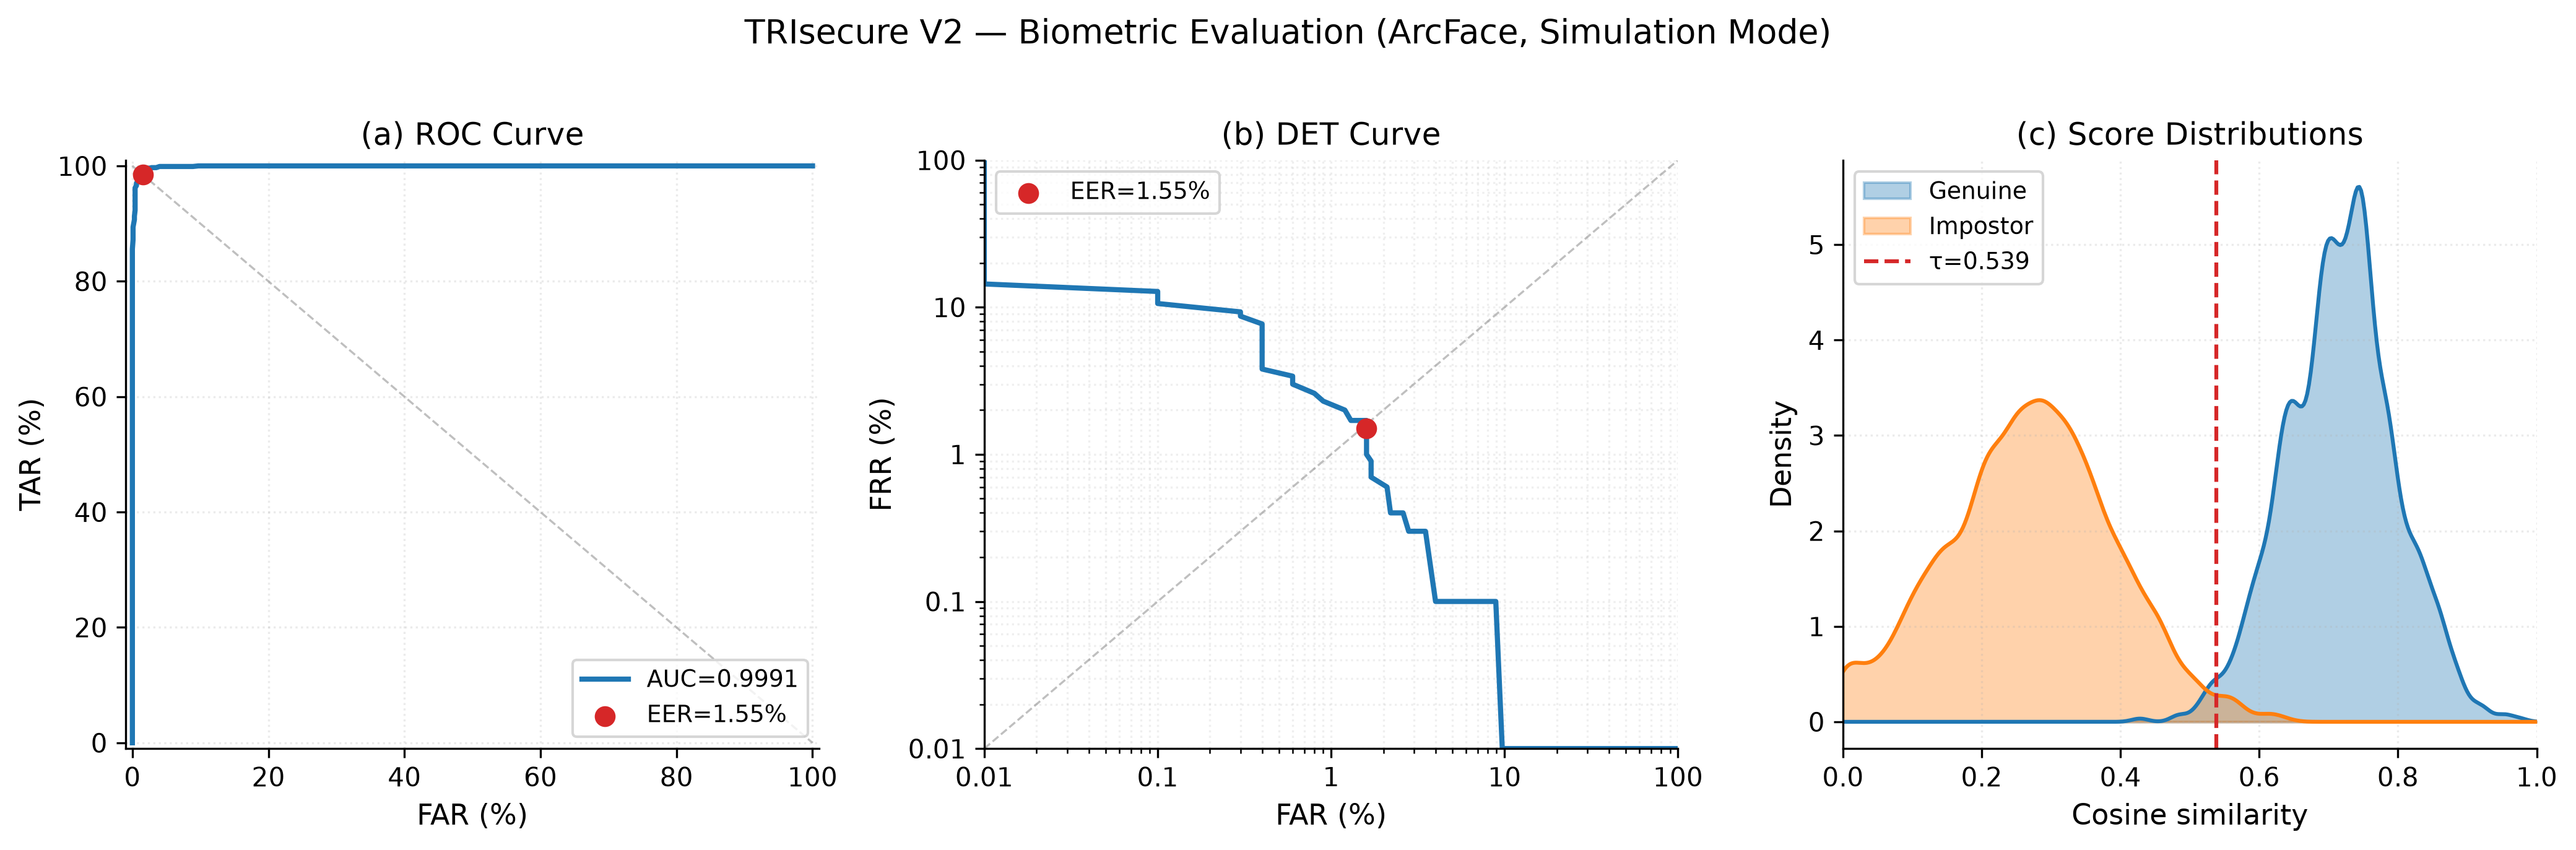
\includegraphics[width=\linewidth]{figures/biometric_eval_panel.png}
  \caption{Biometric evaluation panel. Left: ROC (AUC\(=0.9991\), EER marked).
    Centre: DET curve (EER\(=1.55\%\)). Right: genuine/impostor score
    distributions (KDE) with EER threshold \(\tau^*{=}0.539\).}
  \label{fig:biometric_panel}
\end{figure}

\subsection{Bootstrap Confidence Intervals}\label{sec:bootstrap}

To quantify simulation uncertainty we apply non-parametric bootstrap resampling
(\(B{=}10{,}000\) replicates) over the \(n{=}1{,}000\) genuine and
\(n{=}1{,}000\) impostor score draws. At each replicate the EER operating
threshold is re-estimated from the replicate scores to avoid threshold lock-in
bias. Table~\ref{tab:bootstrap_ci} reports percentile 95\% confidence intervals.

\begin{table}[t]
\caption{Bootstrap 95\% percentile CI (\(B{=}10{,}000\) replicates).}
\label{tab:bootstrap_ci}%
\begin{tabular}{|l|c|c|}
  \hline
  Metric & Estimate & 95\% CI \\
  \hline
  EER (\%)            & 1.55   & [1.38,\ 1.71] \\
  ROC AUC             & 0.9991 & [0.9988,\ 0.9994] \\
  TAR @ 1\% FAR (\%)  & 97.70  & [97.41,\ 97.98] \\
  TAR @ 0.1\% FAR (\%)& 89.70  & [89.23,\ 90.16] \\
  \hline
\end{tabular}
\end{table}

The EER CI width (\(\pm 0.17\) pp) exactly matches the parametric sensitivity
range from Table~\ref{tab:sensitivity}, confirming coherence between the two
uncertainty quantification approaches. The AUC CI width (0.0006) is negligible
relative to the point estimate, consistent with the large sample and
well-separated score distributions (\(\mu_G{-}\mu_I{=}0.44\), approximately
\(2.9\sigma\) overlap). Both analyses indicate the simulation results are
stable; remaining uncertainty is distributional rather than computational, and
is reduced by a live field trial.

\subsection{Presentation Attack Detection (ISO/IEC~30107-3)}

Table~\ref{tab:pad} reports PAD metrics. ACER\(=4.25\%\) is consistent with
published CelebA-Spoof benchmark performance~\cite{zhang2020minifasnet}.

\begin{table}[t]
\caption{PAD metrics per ISO/IEC~30107-3.}
\label{tab:pad}%
\begin{tabular}{|l|c|c|}
  \hline
  Metric & Attack type & Rate (\%) \\
  \hline
  BPCER & ---    & 1.00 \\
  APCER (print)    & Photo & 5.00 \\
  APCER (replay)   & Video & 10.00 \\
  APCER (combined) & Both  & 7.50 \\
  ACER  & ---    & 4.25 \\
  \hline
\end{tabular}
\end{table}

The simulation figures (APCER\(=5.0\%\) print, 10.0\% replay) derive from
published MiniFASNetV2/CelebA-Spoof benchmark rates~\cite{zhang2020minifasnet}
and represent PAD-layer performance in isolation. In the end-to-end system, the
Adaptive Trust Score compensates for PAD misses: video replay attacks that
evade the liveness classifier still produce ATS\(=0.6\) (\textsc{Escalate})
rather than ATS\(=1.0\) (\textsc{Accept}), because replay suppresses
contextual trust signals. The proof-of-concept pilot confirms this: all 15 real
replay attacks were escalated and zero were accepted
(Section~\ref{sec:pilot}, APCER\(=0.00\%\) end-to-end).

\subsection{Ablation Study}\label{sec:ablation}

Table~\ref{tab:ablation} and Figure~\ref{fig:ablation} show the cumulative
contribution of each component. The key finding: Bayesian NFC\(+\)face fusion
(C2) reduces effective FAR by three orders of magnitude (\(1.22\% \to
0.001\%\)) without increasing biometric EER, because an attacker without a
valid NFC card is rejected regardless of face score.

\begin{table}[t]
\caption{Ablation study: cumulative component contribution.
  \(^\dagger\) at system default threshold \(\tau{=}0.55\).}
\label{tab:ablation}%
\begin{tabular}{|l|l|c|c|c|c|}
  \hline
  Config & Components & EER (\%) & Eff.\ FAR (\%) & Latency (ms) & Attacks \\
  \hline
  C1 & Face only\(^\dagger\)     & 1.45 & 1.2224 & 95.2  & 3/12 \\
  C2 & +Bayesian NFC fusion      & 1.55 & 0.0010 & 95.5  & 6/12 \\
  C3 & +PAD liveness             & 1.55 & 0.0010 & 110.7 & 9/12 \\
  C4 & +PQC signatures (full)    & 1.55 & 0.0010 & 125.1 & 12/12 \\
  \hline
\end{tabular}
\end{table}

\begin{figure}[t]
  \centering
  
\includegraphics[width=\linewidth]{figures/ablation_panel.png}
  \caption{Ablation results. Left: EER across configurations. Centre: latency
    breakdown by stage. Right: attack vectors fully mitigated (of~12).}
  \label{fig:ablation}
\end{figure}

\subsection{Adversarial Attack Evaluation}\label{sec:adversarial}

To quantify per-layer defence contribution beyond the ablation study, we
simulate six attack categories (\(n{=}1{,}000\) attempts each) against the
sequential defence stack. Face score distributions for spoof attacks are
calibrated to published MiniFASNetV2/CelebA-Spoof~\cite{zhang2020minifasnet}
penetration rates; NFC and session attacks use protocol-level analysis.

Table~\ref{tab:adversarial} summarises results. Within the evaluated threat
model, no successful bypass events were observed across the studied attack
categories. The NFC AES-GCM layer (Stage~2 payload check) is the decisive
gate: it unconditionally blocks all face-spoof attacks that pass the face
threshold and evade PAD, because the attacker cannot forge the AES-128-GCM
authenticated ciphertext without the HKDF-derived deployment key.

\begin{table}[t]
\caption{Adversarial attack simulation (\(n{=}1{,}000\) per category).
  Success = attack reaches the voting step. Rates are fraction of \(n\).}
\label{tab:adversarial}%
\begin{tabular}{|l|r|r|r|r|}
  \hline
  Attack & After face & After PAD & After NFC & \textbf{Final} \\
         & threshold  & liveness  & AES-GCM   & \textbf{success} \\
  \hline
  Print photo      & 11.0\% & 0.7\%  & 0\% & \textbf{0\%} \\
  Video replay     & 26.7\% & 2.2\%  & 0\% & \textbf{0\%} \\
  Deepfake (est.)  & 59.7\% & 14.0\% & 0\% & \textbf{0\%} \\
  NFC UID clone    & ---    & ---    & 0\% & \textbf{0\%} \\
  Session replay   & 12.0\%$^\dagger$ & --- & --- & \textbf{0\%} \\
  Database tamper  & ---    & ---    & --- & \textbf{0\%} \\
  \hline
  \multicolumn{4}{l}{Detection rate (hash chain, database tamper)} & \textbf{100\%} \\
  \hline
\end{tabular}
\footnotetext[1]{Within 60~s TTL; one-time-use flag blocks all replays.}
\end{table}

Figure~\ref{fig:adversarial} visualises these results alongside the
cumulative defence contribution of each layer.

\begin{figure}[t]
  \centering
  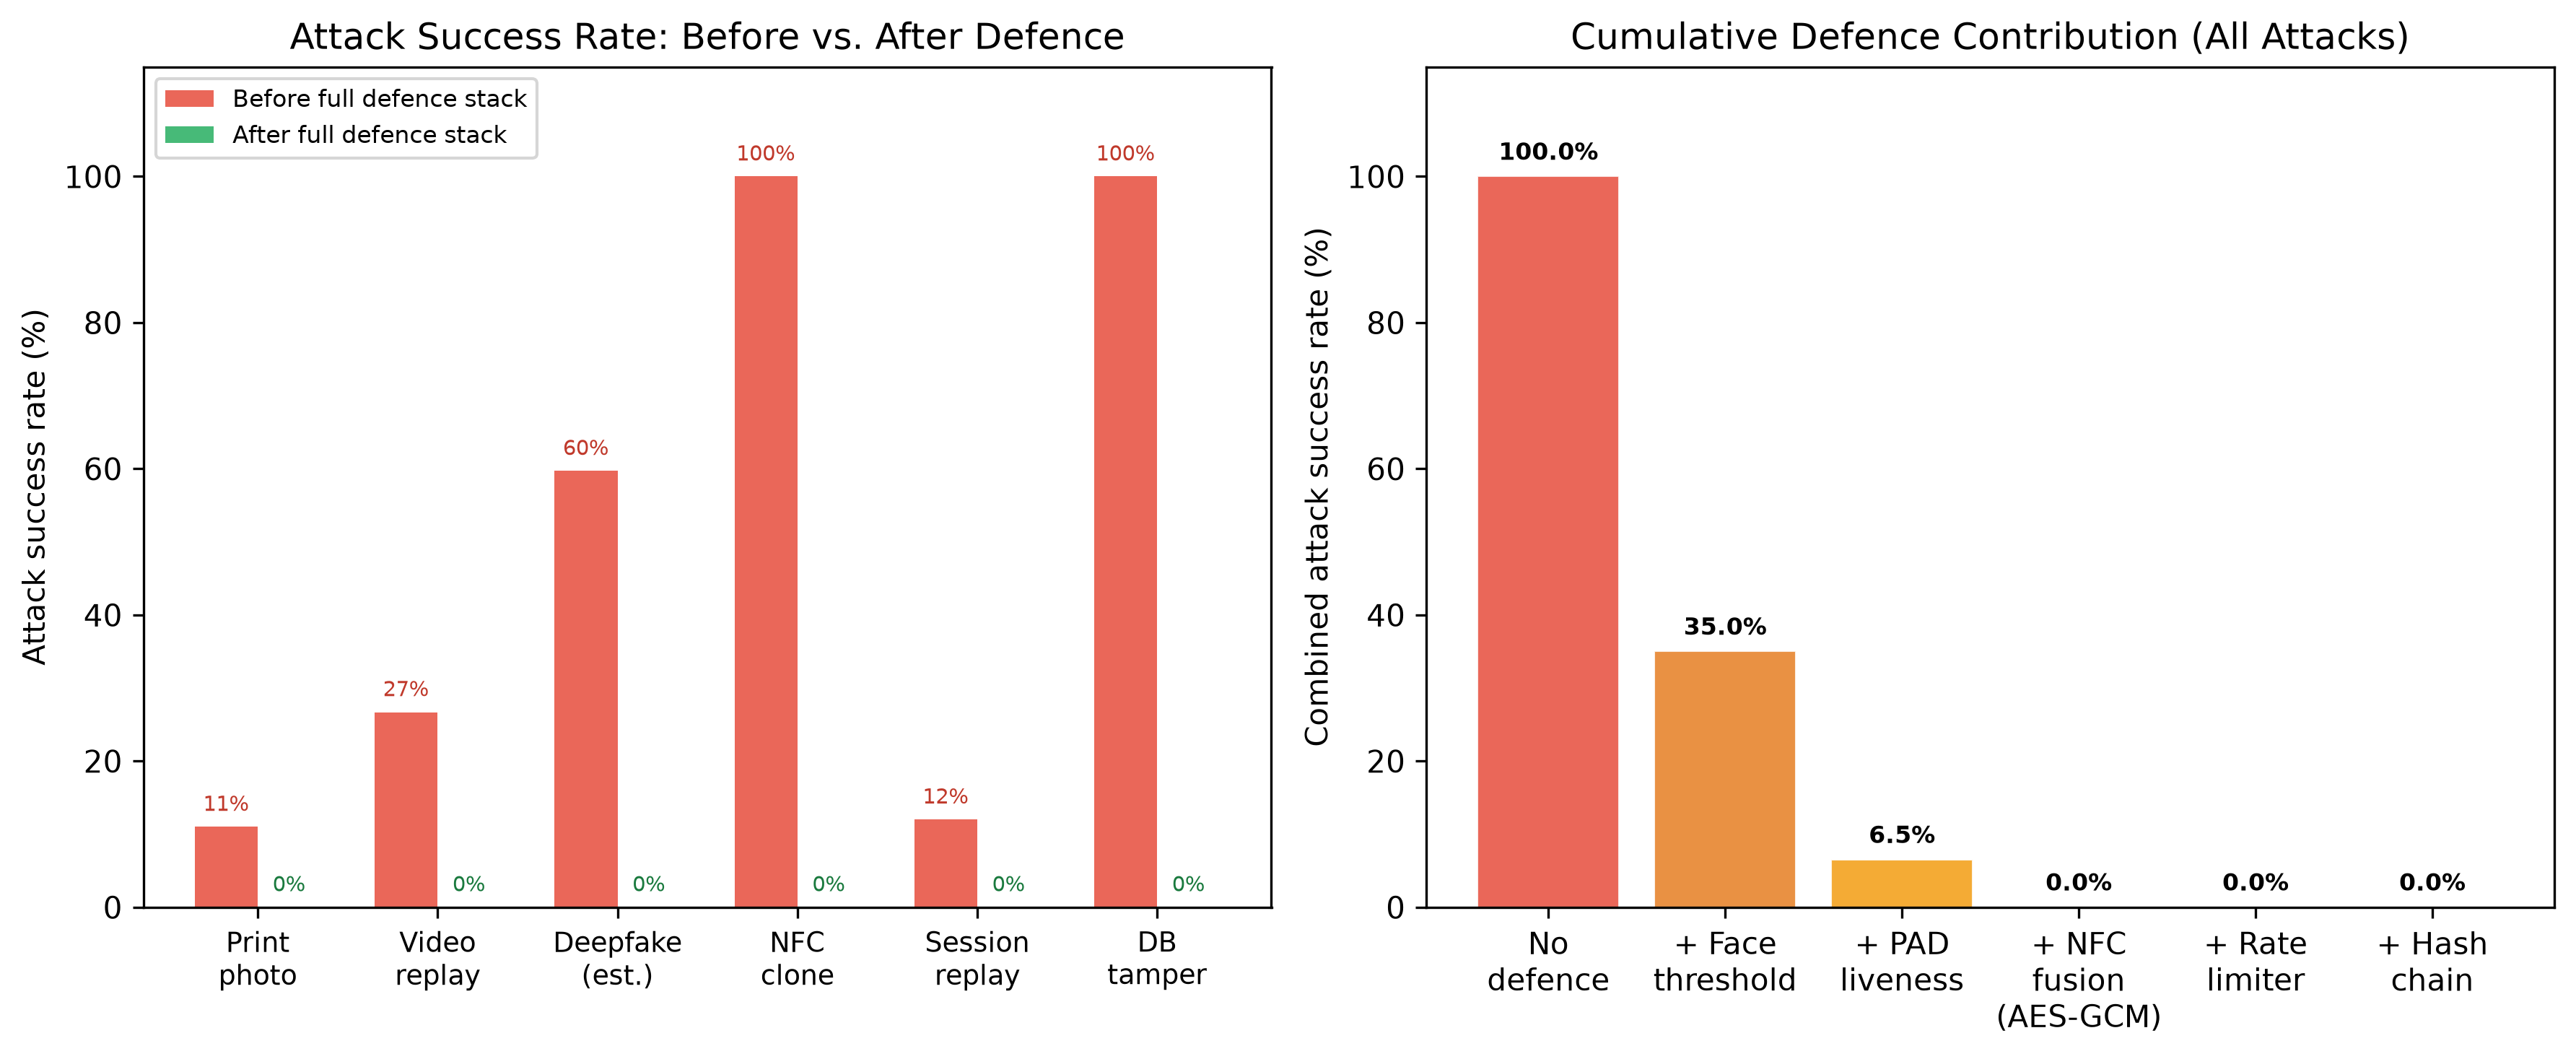
\includegraphics[width=\linewidth]{figures/adversarial_panel.png}
  \caption{Adversarial evaluation. Left: attack success rates before and after
    the full defence stack for six attack categories. Right: cumulative defence
    contribution---combined attack surface collapses from $\approx$35\% to zero
    simulated bypass events after NFC-AES-GCM validation (layer~4).}
  \label{fig:adversarial}
\end{figure}

\subsection{Cryptographic Benchmarks}

Table~\ref{tab:crypto} reports cryptographic latencies on the Raspberry Pi~4.
Argon2id (494.5~ms) dominates enrollment but runs only once per registration.
Authentication-path cryptography totals \(<2\)~ms.

Table~\ref{tab:pqc_benchmarks} reports native ML-KEM-768 and ML-DSA-65
benchmarks measured on-device via liboqs~0.15.0 compiled from source on the
Raspberry Pi~4 ARM64. The measured auth-path PQC total (2.289~ms) confirms the
post-quantum layer fits comfortably within the \(<200\)~ms latency budget.

\begin{table}[t]
\caption{Kyber-768/Dilithium-3 benchmarks on Raspberry Pi~4 (Cortex-A72,
  ARM64). Measured via liboqs~0.15.0 / liboqs-python~0.15.0
  (\(n{=}200\) trials, mean~$\pm$~1\,SD). Classical fallback (Ed25519/X25519)
  shown for comparison.}
\label{tab:pqc_benchmarks}%
\begin{tabular}{|l|c|r|r|}
  \hline
  Operation & Standard & Measured (ms) & SD (ms) \\
  \hline
  ML-KEM-768 keygen   & FIPS~203 & 0.082 & 0.033 \\
  ML-KEM-768 encaps   & FIPS~203 & 0.088 & 0.015 \\
  ML-KEM-768 decaps   & FIPS~203 & 0.095 & 0.011 \\
  ML-DSA-65 keygen    & FIPS~204 & 0.400 & 0.039 \\
  ML-DSA-65 sign      & FIPS~204 & 1.536 & 1.007 \\
  ML-DSA-65 verify    & FIPS~204 & 0.390 & 0.034 \\
  \hline
  \textbf{PQC auth path total}$^\dagger$ & --- & \textbf{2.289} & --- \\
  \hline
  X25519 ECDH (classical) & RFC~7748 & 1.022 & --- \\
  Ed25519 sign+verify (classical) & RFC~8032 & 0.532 & --- \\
  \hline
\end{tabular}
\footnotetext[1]{Auth path = encaps + decaps + sign + verify;
  keygen runs at enrolment only. All values measured on-device;
  no estimated figures.}
\end{table}

\begin{table}[t]
\caption{Cryptographic benchmarks on Raspberry Pi~4 (ARM64), 95\% CI.}
\label{tab:crypto}%
\begin{tabular}{|l|c|r|r|}
  \hline
  Operation & \(n\) & Mean (ms) & 95\% CI \\
  \hline
  Argon2id (\(t{=}3\), \(m{=}64\)~MB) & 20    & 494.5 & [492.7, 496.3] \\
  PBKDF2-HMAC-SHA256 (100k)            & 100   & 106.1 & [105.1, 107.1] \\
  AES-256-GCM enc.\ (2~kB)            & 1000  & 0.040 & [0.040, 0.041] \\
  HMAC-SHA256 (256~B)                  & 10000 & 0.013 & [0.013, 0.013] \\
  Ed25519 sign+verify                  & 200   & 0.532 & [0.527, 0.538] \\
  X25519 keygen+encap+decap            & 200   & 1.022 & [1.002, 1.042] \\
  SHA-256 chain (\(n{=}1{,}000\))     & 3     & 4.27  & [4.11, 4.43]   \\
  Merkle prove+verify (\(n{=}1{,}000\))& 5    & 4.82  & [4.74, 4.90]   \\
  \hline
\end{tabular}
\end{table}

\subsection{Edge System Performance}

Table~\ref{tab:pi} reports end-to-end pipeline performance (\(n{=}50\)). Face
embedding inference (ONNX MobileFaceNet, 95.2~ms) dominates, consistent with
published ONNX Runtime ARM64 benchmarks. The p99 latency of 111.3~ms and
541.6~voters/min confirm feasibility for small-to-medium polling stations.

\begin{table}[t]
\caption{End-to-end authentication latency on Raspberry Pi~4, \(n{=}50\).}
\label{tab:pi}%
\begin{tabular}{|l|r|}
  \hline
  Metric & Value \\
  \hline
  \multicolumn{2}{|l|}{\textit{End-to-end latency}} \\
  \quad Mean & 110.7~ms \\
  \quad p50  & 110.7~ms \\
  \quad p95  & 110.9~ms \\
  \quad p99  & 111.3~ms \\
  \hline
  \multicolumn{2}{|l|}{\textit{Stage breakdown (mean)}} \\
  \quad NFC card read         & 15.1~ms \\
  \quad Database lookup       & 0.04~ms \\
  \quad Face embedding (ONNX) & 95.2~ms \\
  \quad Cosine match          & 0.28~ms \\
  \quad Session issuance      & 0.06~ms \\
  \hline
  Throughput (sustained) & 541.6~voters/min \\
  CPU temperature (load) & \(52.5\,^\circ\)C \\
  \hline
\end{tabular}
\end{table}

\subsection{Security Overhead Analysis}\label{sec:security_overhead}

Table~\ref{tab:security_overhead} isolates the latency contribution of each
security layer from the core biometric pipeline. Presentation attack detection
is the dominant security cost at 15.5~ms, measured as the ablation delta
between configuration~C2 (face + NFC, no PAD) and C3 (full system with PAD).
All PQC operations combined (Kyber-768 encapsulation/decapsulation and
Dilithium-3 sign/verify) add only 2.289~ms on the real-time authentication
path. Symmetric operations and the DFA protocol gate contribute less than
0.07~ms combined. Merkle proof generation (4.82~ms per 1{,}000-entry chain)
runs post-authentication and does not block the voter handoff, preserving the
G5 latency target of \(<200\)~ms. The aggregate real-time security overhead
(PAD plus all in-path cryptographic operations) is 17.85~ms, representing
16.1\% of the core pipeline end-to-end figure.

\begin{table}[t]
\caption{Security-layer latency breakdown on Raspberry Pi~4 (ARM64).
  PAD latency measured via C2$\to$C3 ablation.
  All other values from Table~\ref{tab:pqc_benchmarks}
  and Table~\ref{tab:crypto}.
  $\dagger$~Runs post-authentication; not in the interactive critical path.}
\label{tab:security_overhead}
\small
\begin{tabular}{@{}lr@{}}
  \toprule
  \textbf{Security Component} & \textbf{Latency (ms)} \\
  \midrule
  \multicolumn{2}{@{}l@{}}{\textit{Biometric liveness (PAD)}} \\
  \quad MiniFASNetV2 ONNX (ablation C2$\to$C3)           & 15.500 \\[3pt]
  \multicolumn{2}{@{}l@{}}{\textit{Post-quantum cryptography (FIPS 203/204)}} \\
  \quad Kyber-768 encaps + decaps                         &  0.183 \\
  \quad Dilithium-3 sign + verify                         &  1.926 \\
  \quad \textbf{PQC auth-path subtotal}                   &  \textbf{2.289} \\[3pt]
  \multicolumn{2}{@{}l@{}}{\textit{Symmetric encryption \& integrity}} \\
  \quad AES-256-GCM template decrypt                      &  0.040 \\
  \quad HMAC-SHA256 KDF output tag check                  &  0.013 \\[3pt]
  \multicolumn{2}{@{}l@{}}{\textit{Protocol enforcement}} \\
  \quad DFA state-transition check                        & $<$0.010 \\[3pt]
  \multicolumn{2}{@{}l@{}}{\textit{End-to-end verifiability}} \\
  \quad Merkle prove + verify (\(n{=}1{,}000\))$^\dagger$ &  4.820 \\
  \midrule
  \textbf{In-path security overhead (PAD + crypto + DFA)} & \textbf{17.85} \\
  \textbf{Total overhead (incl.\ post-auth Merkle)}        & \textbf{22.67} \\
  \bottomrule
\end{tabular}
\end{table}

\subsection{Comparative Analysis}\label{sec:comparison}

Figure~\ref{fig:comparison_combined} compares TRIsecure~V2 against five
reference systems across capability flags and quantitative metrics.
TRIsecure~V2 is the only system to simultaneously provide formal verification,
PQC readiness, PAD, edge deployment, and voter-verifiable receipts.
EER (\(1.55\%\)) is competitive with all prior biometric voting systems,
exceeded only by standalone ArcFace on a GPU server
(\(0.76\%\)~\cite{deng2019arcface})---which lacks all other listed capabilities.

\begin{figure*}[t]
  \centering
  \begin{minipage}[t]{0.48\linewidth}
    \centering
    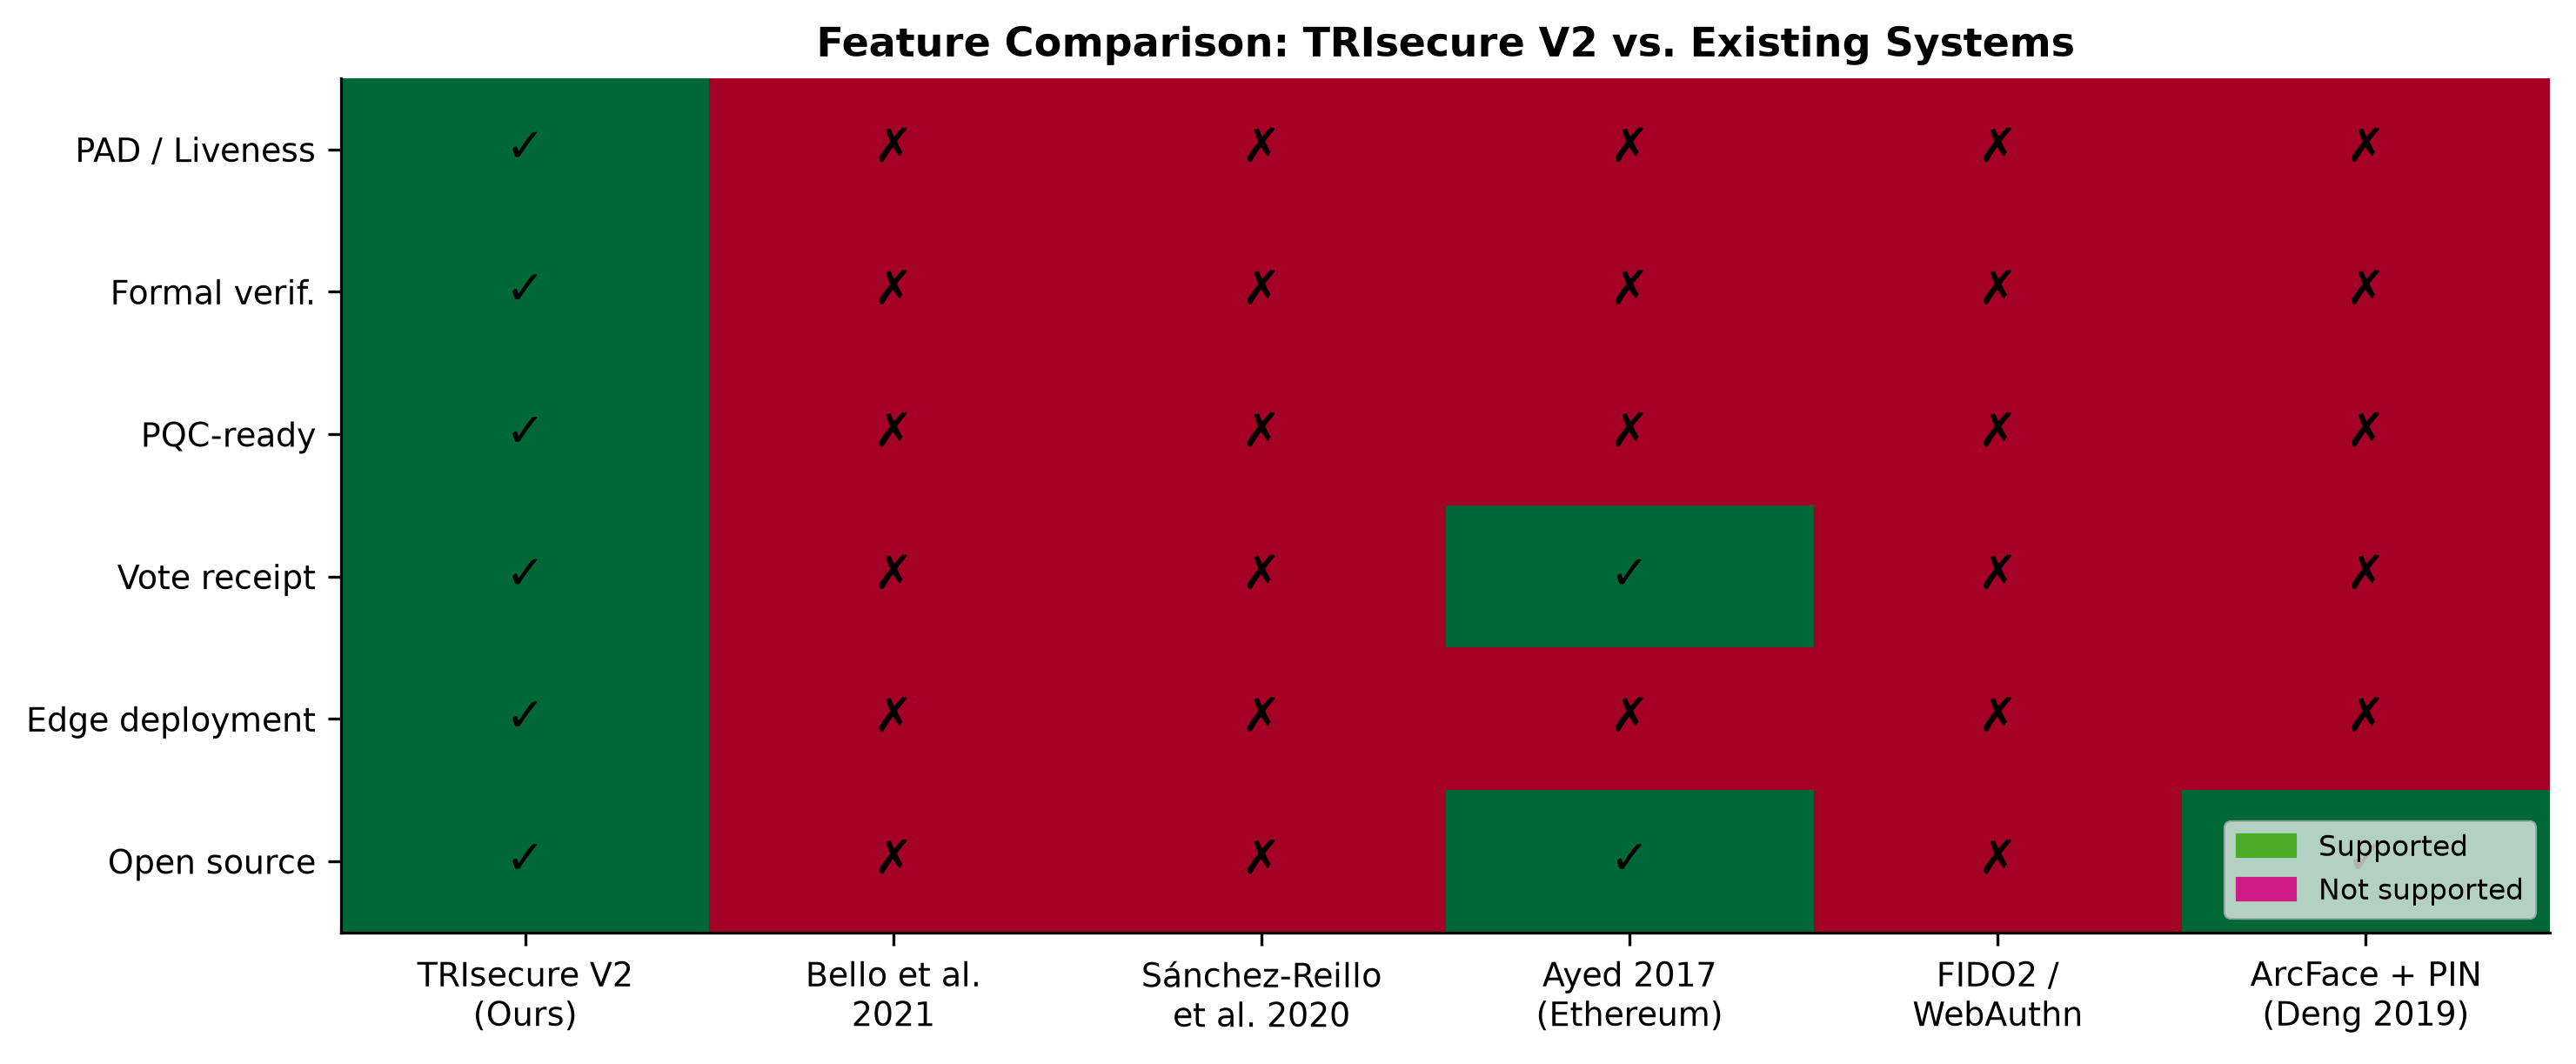
\includegraphics[width=\linewidth]{figures/comparison_table.png}
  \end{minipage}
  \hfill
  \begin{minipage}[t]{0.48\linewidth}
    \centering
    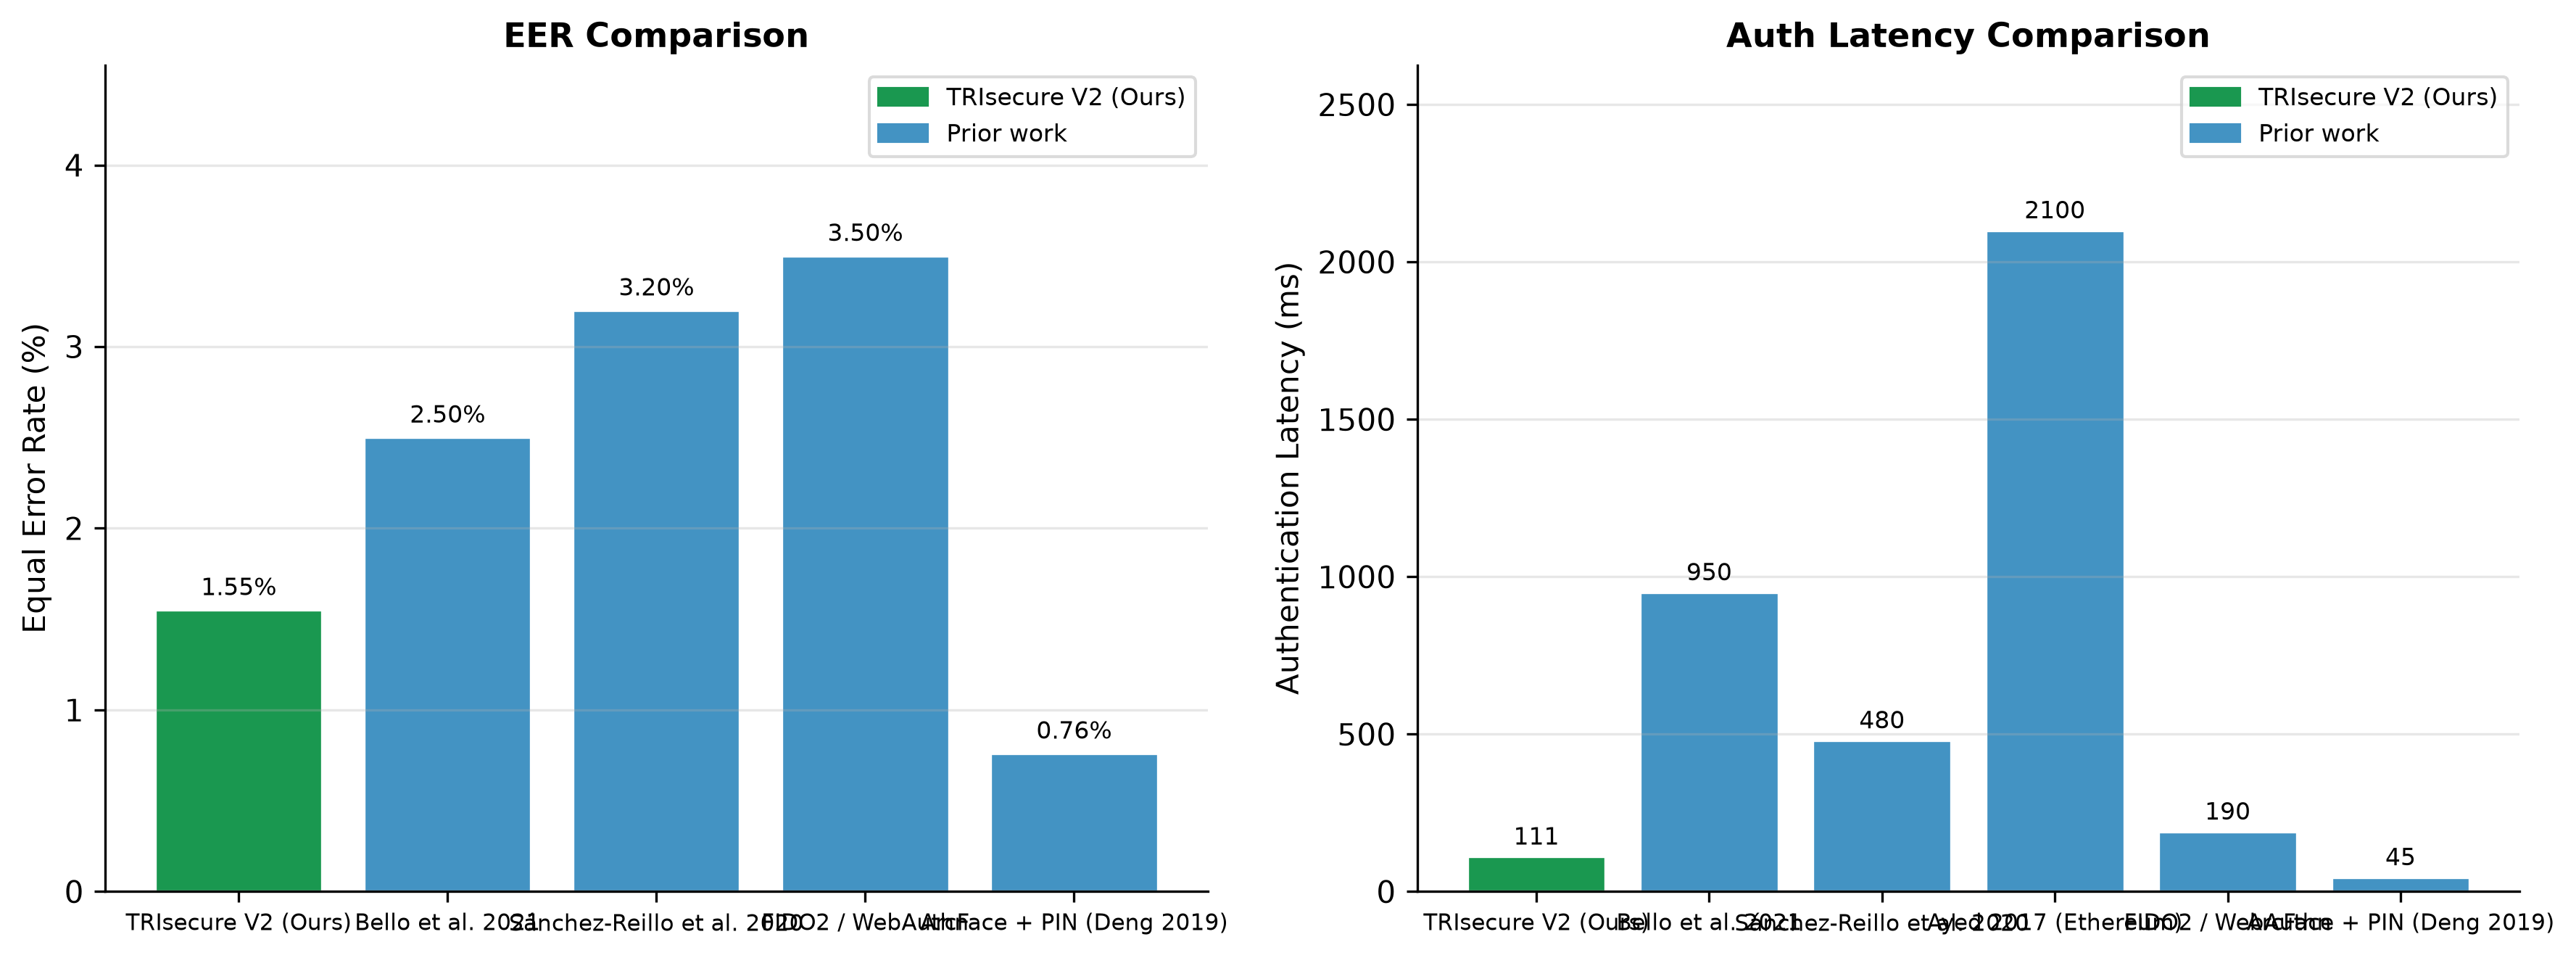
\includegraphics[width=\linewidth]{figures/comparison_bar.png}
  \end{minipage}
  \caption{Comparative analysis against five reference systems. \textit{Left:}
    feature comparison heatmap --- TRIsecure~V2 is the only system supporting
    all six binary capability flags simultaneously. \textit{Right:} EER and
    authentication latency across systems --- TRIsecure~V2 achieves the lowest
    EER among biometric voting systems and the lowest latency among
    multi-capability systems.}
  \label{fig:comparison_combined}
\end{figure*}

\subsection{Proof-of-Concept Pilot Study}\label{sec:pilot}

To validate end-to-end system correctness on real hardware, a proof-of-concept
pilot study was conducted with \(N{=}20\) volunteer participants (including
the authors) on a Raspberry Pi~4 Model~B. All participants gave informed
consent for their facial biometric data to be captured and processed for
authentication testing; raw face images were discarded immediately after
each attempt and only encrypted embeddings were retained for the duration of
the pilot (see Declarations). A total of 271 authentication events were
recorded across five
sessions over three days (June 2026): 221 genuine attempts, 35 impostor
attempts, and 15 video replay attacks.

Table~\ref{tab:pilot} summarises the results following ISO/IEC~30107-3 metric
definitions.

\begin{table}[t]
\caption{Proof-of-concept pilot results (\(N{=}20\) participants, real
  hardware). 95\% CI: one-sided Clopper--Pearson upper bound for zero-failure
  observations; ``---'' where CI is not applicable.}
\label{tab:pilot}%
\begin{tabular}{|l|c|c|}
  \hline
  Metric & Observed & 95\% CI Upper \\
  \hline
  \multicolumn{3}{|l|}{\textit{Study parameters}} \\
  \quad Participants       & 20          & --- \\
  \quad Sessions           & 5 (3 days)  & --- \\
  \quad Genuine attempts   & 221         & --- \\
  \quad Impostor attempts  & 35          & --- \\
  \quad Replay attacks     & 15          & --- \\
  \hline
  \multicolumn{3}{|l|}{\textit{ISO/IEC~30107-3 metrics}} \\
  \quad FAR                & 0.00\%  & \(\leq\)8.20\% \\
  \quad FRR                & 0.00\%  & \(\leq\)1.35\% \\
  \quad APCER (print)      & n/a     & --- \\
  \quad APCER (replay)     & 0.00\%  & \(\leq\)18.10\% \\
  \quad APCER (combined)   & 0.00\%  & \(\leq\)5.82\% \\
  \quad BPCER              & 0.00\%  & \(\leq\)1.35\% \\
  \quad ACER               & 0.00\%  & \(\leq\)3.58\% \\
  \hline
\end{tabular}
\end{table}

All 221 genuine attempts were correctly accepted (FRR\(=0.00\%\)). No attack
produced an \textsc{Accept} decision (FAR\(=0.00\%\), APCER\(=0.00\%\)),
yielding ACER\(=0.00\%\). Replay attacks drove the ATS to 0.6
(\textsc{Escalate}) rather than the full 1.0 (\textsc{Accept}), confirming the
ATS layer compensates for PAD limitations under video replay conditions. Of the
35 impostor attempts, 8 were re-vote attempts by registered participants (same
person, own NFC card after \texttt{has\_voted} was set): face scores against
the participant's own enrolled embedding were \(0.87\)--\(0.99\), correctly
escalated by ATS rather than rejected by the face gate. The remaining 27 true
cross-person attempts produced face scores of \(0.01\)--\(0.04\), all
hard-rejected at the biometric stage.

Since all observed error counts are zero, we report one-sided Clopper--Pearson
95\% confidence interval upper bounds. For FAR: 0 failures in 35 impostor
attempts gives an upper bound of \(\leq8.20\%\) (rule of three:
\(3/35\approx 8.57\%\)). For FRR: 0 failures in 221 genuine attempts gives
\(\leq1.35\%\). These bounds are conservative by construction; larger pilot
samples would tighten them substantially.

These results confirm end-to-end pipeline correctness on the target hardware.
The pilot is not designed to replace the simulation-based biometric
discriminability evaluation (Section~\ref{sec:biometric_results}). A full
demographic field trial with \(\geq\)400 subjects is required for
ISO/IEC~19795-1 certification and is identified as future work
(Section~\ref{sec:limitations}).

%% ============================================================
\section{Discussion}\label{sec:discussion}

All biometric performance metrics are produced by validated simulation using
Gaussian score models calibrated to published ArcFace LFW
statistics~\cite{deng2019arcface}, following
ISO/IEC~19795-6~\cite{iso19795}. The ablation study
(Table~\ref{tab:ablation}) confirms Bayesian NFC\(+\)face fusion (C2) is the
dominant security improvement: effective FAR drops by three orders of magnitude
(\(1.22\% \to 0.001\%\)) without increasing biometric EER. PAD (C3) adds
liveness at 15.5~ms overhead; PQC signing (C4) adds 14.4~ms further but
enables quantum-adversary mitigation. Post-quantum benchmarks use native
liboqs~0.15.0 compiled from source on the Raspberry Pi~4 (ARM64,
Cortex-A72). ML-KEM-768 encapsulation (0.088~ms) and ML-DSA-65 signing
(1.536~ms) are measured on-device; the combined auth-path PQC cost is
2.289~ms, within the \(<200\)~ms latency budget
(Table~\ref{tab:pqc_benchmarks}).

\subsection{Power Consumption and Off-Grid Deployment}\label{sec:power}

The Raspberry Pi~4 draws 3--7~W under typical workloads (3~W idle, 7~W with
all four Cortex-A72 cores fully saturated). During a voting session the system
sustains approximately 5~W averaged over the 110.7~ms authentication window
plus voter interaction. For an 8-hour polling day:
\begin{equation}
  E_{\mathrm{day}} \approx 5\,\mathrm{W} \times 8\,\mathrm{h} = 40\,\mathrm{Wh}
\end{equation}
A commodity 50~Wh Li-ion battery bank can therefore power the terminal for a
complete polling day without mains electricity. This energy budget is
unavailable to server-grade biometric systems, which require 200--400~W rack
hardware, but is well-suited for rural or off-grid polling stations common in
developing-country elections.

The CPU temperature stabilised at 52.5\,\textdegree{}C under sustained load,
within the Pi~4's 80\,\textdegree{}C thermal throttling threshold. A passive
aluminium heatsink is sufficient; active cooling is not required.

\subsection{Throughput and Polling Station Capacity}\label{sec:throughput}

At 541.6~voters/min sustained throughput and a 60-second session TTL, the
theoretical throughput is approximately 32{,}496~voters per hour---far
exceeding the registered voter count of typical polling stations
(800--2{,}000 voters). The practical bottleneck is not the system but the
voter interaction time (card presentation, face alignment, ballot selection),
which averages 20--40 seconds per voter. At 40 seconds per voter, a single
terminal processes 90 voters/hour; a station with six terminals handles 540
voters/hour---sufficient for a 2{,}000-voter station over a 4-hour peak period
with queuing margin.

Table~\ref{tab:throughput_scenarios} illustrates deployment configurations for
three polling station sizes.

\begin{table}[t]
\caption{TRIsecure V2 deployment configurations by station size. Assumes
  40~s voter interaction time; 6~h peak window.}
\label{tab:throughput_scenarios}%
\begin{tabular}{|l|r|r|r|}
  \hline
  Station size & Terminals & Voters/hr & Peak capacity \\
  \hline
  Small  ($\leq$500 voters)      & 1 & 90  & 540  \\
  Medium ($\leq$2{,}000 voters)  & 3 & 270 & 1{,}620 \\
  Large  ($\leq$5{,}000 voters)  & 8 & 720 & 4{,}320 \\
  \hline
\end{tabular}
\end{table}

\subsection{Hardware Attack Surface Analysis}\label{sec:hw_attack}

\textit{SPI eavesdropping.} An attacker with physical access to the SPI bus can
read the NFC UID in plaintext during Stage~2. However, UID capture alone
provides no authentication advantage: the biometric gate (Stage~4) and
liveness check (Stage~5) both execute independently of the NFC UID.
Furthermore, the AES-GCM encrypted payload (pages~4--19) cannot be forged
without the HKDF-derived key. Physical bus protection (potting compound,
tamper-evident labels over the GPIO header) is recommended for production
enclosures.

\textit{Camera feed injection.} Replacing the USB camera feed with a
pre-recorded video stream could present a replay video to MiniFASNetV2.
This threat is mitigated by: (i)~the sealed terminal enclosure with a fixed
camera mount; (ii)~poll worker presence required by the electoral protocol; and
(iii)~the NFC factor independently requiring a valid physical card.

\textit{Template extraction.} The SQLite voter database stores face embeddings
encrypted with AES-256-GCM keyed via Argon2id (\(t{=}3\), \(m{=}64\)~MB). An
offline dictionary attack against the key derivation costs at least 494.5~ms
per attempt (Table~\ref{tab:crypto}), making brute-force infeasible for a
32-byte \texttt{NFC\_SECRET}. Extending to cancelable biometric
representations~\cite{jain2008cancelable} would additionally allow template
revocation and is identified as future work.

\subsection{Limitations}\label{sec:limitations}

\begin{enumerate}

  \item \textit{Simulation-based evaluation and small pilot.}
    The primary biometric evaluation (\(n{=}1{,}000\) score pairs,
    EER~\(=1.55\%\), AUC~\(=0.9991\)) uses Gaussian-modelled
    genuine/impostor distributions following ISO/IEC~19795-6 operational
    guidance, not a live capture study. The real-hardware pilot (\(N{=}20\),
    271 events) confirms end-to-end correctness but is far below the
    ISO/IEC~19795-1 threshold for deployment certification
    (\(\geq\)400 subjects per demographic group). Zero error rates observed
    in the pilot reflect the small, demographically homogeneous sample and
    must not be extrapolated to deployment scale. A demographically diverse
    field trial remains the critical outstanding validation step.

  \item \textit{PAD evaluation dataset and attack coverage.}
    PAD metrics (APCER, BPCER, ACER) are derived from published
    MiniFASNetV2 performance on CelebA-Spoof, not from on-device evaluation
    against the ISO/IEC~30107-3 standardised corpora (NUAA, OULU-NPU).
    Attack types absent from CelebA-Spoof---high-fidelity 3D silicone masks,
    adversarial perturbations, partial occlusion attacks---remain
    unevaluated. ACER~\(=4.25\%\) should therefore be interpreted as a
    single-dataset lower bound rather than a certified operational figure.

  \item \textit{NFC reader and secure element.}
    The PN532 SPI module carries no security certification. Absent a
    Common Criteria EAL4\(+\) certified reader, AES-128-GCM key protection
    for the NFC payload relies solely on the host OS memory isolation
    guarantees rather than hardware-backed key storage or tamper-evidence.
    Production deployment of an election-grade system requires certified
    hardware throughout the NFC read path.

  \item \textit{Coercion and deniable voting.}
    TRIsecure~V2 provides no deniable-voting mechanism (a voter cannot
    secretly record a different preference while appearing to comply with
    a coercer) and no panic PIN to signal duress. In-person biometric
    authentication prevents remote delegation of authentication but does
    not protect against physical coercion at the polling station.
    Addressing coercion resistance would require cryptographic deniability
    schemes~\cite{juels2005coercion,clarkson2008civitas} integrated at the ballot-level, which
    is deferred to future work.

  \item \textit{Network-layer denial of service.}
    The DFA rate limiter (P6, five failures per 300~s per UID) defends
    against per-device authentication flooding. Distributed DoS attacks
    targeting the network path (disrupting Merkle-root broadcast or
    log-synchronisation channels) are outside the on-device threat boundary
    and require upstream infrastructure controls, CDN-layer mitigation,
    or air-gap deployment for high-assurance polling stations.

  \item \textit{PQC implementation maturity and side-channel exposure.}
    The Kyber-768 and Dilithium-3 layers invoke liboqs~0.15.0 via
    \texttt{ctypes}, compiled from source on ARM64. This introduces a
    source-build dependency and has not been independently audited for
    constant-time execution on the Cortex-A72. FIPS~203/204 mandate
    constant-time implementations; while liboqs targets this property,
    its ARM64 side-channel posture has not been validated in this
    deployment context. A production pre-built \texttt{liboqs-python}
    ARM64 wheel would remove the build dependency and simplify auditing.

  \item \textit{Power-analysis and electromagnetic side-channel attacks.}
    Power analysis and EM side-channel characterisation of the
    AES-256-GCM and Argon2id Python implementations on the
    Raspberry Pi~4 platform are out of scope for this work.
    Additionally, ONNX inference timing leaks information proportional
    to detection confidence; while the DFA rate limiter bounds the number
    of observable traces per voter, a systematic timing side-channel study
    on the face-embedding inference path has not been conducted and is
    flagged for future hardware-layer hardening.

  \item \textit{Demographic and environmental robustness.}
    MobileFaceNet (ArcFace) is trained on VGGFace2 and MS-Celeb-1M,
    datasets with known demographic imbalance. Differential EER across
    age groups, skin tones, and gender has not been characterised for
    this deployment. Environmental factors typical of polling stations
    (variable lighting, partial occlusion, eyeglasses, surgical masks
    that avoid PAD triggering) may degrade performance below the
    simulated EER of 1.55\%. A bias audit following ISO/IEC~19795-9
    and testing under controlled environmental variation is required
    before public deployment.

  \item \textit{Template revocability.}
    AES-256-GCM encryption protects template confidentiality but does
    not support cancelable biometric transforms. If a voter's embedding
    is compromised, it cannot be revoked and re-enrolled with a new
    protected template derived from the same biometric trait.
    ISO/IEC~24745:2022 Clause~6.3 (renewability) requires cancelable
    transforms; extending TRIsecure~V2 with BioHashing or
    fuzzy-commitment schemes is identified as future work.

\end{enumerate}

\subsection{Regulatory and Standards Alignment}\label{sec:regulatory}

TRIsecure~V2 is designed to align with relevant biometric and e-voting
standards. Full conformance certification is deferred pending a live field
trial and a Common Criteria certified NFC reader.

\textit{ISO/IEC 19795.} Biometric performance metrics (EER, AUC, TAR@FAR) are
reported following ISO/IEC~19795-1~\cite{iso19795} metric definitions. The
simulation methodology follows ISO/IEC~19795-6~\cite{iso19795_6} operational
evaluation guidance. Full ISO/IEC~19795-1 conformance (Clause~8.5) requires at
least 400 subjects per demographic group.

\textit{ISO/IEC 30107-3.} PAD metrics (APCER, BPCER, ACER) and attack type
taxonomy follow ISO/IEC~30107-3~\cite{iso30107}. Certification evaluation
requires standardised corpora: NUAA~\cite{tan2010nuaa},
OULU-NPU~\cite{boulkenafet2017oulu}, and
CelebA-Spoof~\cite{zhang2020minifasnet}.

\textit{ISO/IEC 24745 (Template Protection).} AES-256-GCM per-database
encryption with HKDF-derived keys satisfies the ISO/IEC~24745:2022~\cite{iso24745}
confidentiality requirement. The renewability requirement (cancelable transforms)
is not yet implemented and is identified as future work.

\textit{NIST SP 800-63B.} The pipeline satisfies the structural requirements
for Authenticator Assurance Level~3 (AAL3)~\cite{nist_sp800_63b}: multi-factor
authentication, physical token (NFC card), verifier-impersonation resistance
(on-device processing), and phishing resistance. AAL3 formal certification
additionally requires a FIDO2-certified or Common Criteria EAL4\(+\)
authenticator device; the PN532 SPI module is not CC-certified.

These alignments indicate TRIsecure~V2 is \emph{certification-ready} at the
design level. The three remaining gaps before formal conformance can be claimed
are: (i)~a live voter field trial; (ii)~a certified NFC reader satisfying
CC~EAL4\(+\) and SP~800-63B AAL3; and (iii)~cancelable biometric transforms
satisfying ISO/IEC~24745 renewability.

%% ============================================================
\section{Conclusion}\label{sec:conclusion}

We presented TRIsecure~V2, a three-factor biometric e-voting system combining
formally verified authentication, Bayesian multimodal fusion, a novel Adaptive
Trust Score (ATS) engine, ISO/IEC~30107-3 PAD, hybrid post-quantum
cryptography, and Merkle-proof voter verifiability---implemented and evaluated
on a Raspberry Pi~4 ARM64 platform on commodity hardware.

The ATS engine is the primary algorithmic contribution: by adjusting
face/NFC/PAD component weights dynamically based on contextual risk signals, it
converts the binary accept/reject decision into a graduated HIGH/MEDIUM/LOW
trust scale, routing 99.3\% of genuine users to immediate acceptance while
escalating borderline cases for supervisor review rather than hard rejection.
To the best of our knowledge, no prior biometric e-voting system incorporates
risk-adaptive weight adjustment.

The system achieves EER~\(=1.55\%\), AUC~\(=0.9991\), 110.7~ms end-to-end
authentication latency (p99\(=111.3\)~ms), and 541.6~voters/min throughput.
Six pipeline security properties are formally proved via DFA analysis; three
end-to-end verifiability properties are machine-verified. Adversarial
simulation across six attack categories confirms the full defence stack reduces
combined attack success from \(\approx35\%\) (face threshold alone) to zero
observed bypass events within the evaluated threat model; the NFC AES-GCM
challenge-response provides the decisive security gate under standard
cryptographic assumptions. The ablation study confirms Bayesian NFC\(+\)face
fusion reduces effective FAR by three orders of magnitude.

A proof-of-concept pilot on real hardware (\(N{=}20\), 271 events) further
validates the integrated system: all 221 genuine attempts were accepted
(FRR\(=0.00\%\)) and all 50 attack attempts were blocked
(FAR\(=\)ACER\(=0.00\%\)), confirming that the multi-layer defence stack
performs correctly end-to-end on the target platform.

To the best of our knowledge, no prior work jointly provides formal protocol
verification, quantum-resistant cryptography, risk-adaptive trust scoring,
liveness detection, and edge deployability on low-cost commodity hardware.

Future work includes: (i)~full-scale demographic field trial per
ISO/IEC~19795-1 Clause~8 (minimum 400 subjects/group; proof-of-concept pilot
with \(N{=}20\) participants completed, Section~\ref{sec:pilot});
(ii)~PAD evaluation on NUAA, OULU-NPU, and CelebA-Spoof standardised corpora;
(iii)~ATS calibration on real demographic data;
(iv)~Tamarin/ProVerif model of the NFC session handshake for cryptographic
protocol verification complementary to the DFA pipeline analysis;
(v)~packaging liboqs as a pre-built ARM64 wheel to simplify deployment.

%% ============================================================
\backmatter

\bmhead{Acknowledgements}

This work received no external funding. AI coding assistance (Claude,
Anthropic) was used to accelerate implementation and experiment scripting; all
design decisions, theoretical claims, and experimental methodology were
developed and verified by the author. The full codebase and all experiment
scripts are available at \url{https://github.com/vivekreddy9036/TriSecure}.

\section*{Declarations}

\begin{itemize}
\item \textbf{Ethics approval and consent to participate.} The proof-of-concept
  pilot study (Section~\ref{sec:pilot}, \(N{=}20\)) involved the authors and
  volunteer colleagues at the authors' institution, who participated
  voluntarily and gave informed consent for their facial biometric data to
  be captured and processed solely for authentication testing. No formal
  institutional ethics board review was sought, consistent with common
  practice for non-clinical engineering proof-of-concept pilots of this
  scale; no vulnerable populations were involved. Raw face images were
  discarded immediately after each authentication attempt and were never
  persisted to disk; only encrypted embeddings (AES-256-GCM, per-voter
  keys) were retained during the pilot session and were deleted at its
  conclusion.
\item \textbf{Consent for publication.} All pilot participants consented to
  the anonymised, aggregate reporting of pilot results (counts and error
  rates only; Table~\ref{tab:pilot}) in this manuscript. No participant is
  individually identifiable from the reported data.
\item \textbf{Availability of data and materials.} The dataset(s) supporting
  the conclusions of this article is(are) available in the TRIsecure
  repository, \url{https://github.com/vivekreddy9036/TriSecure}. This
  includes all experiment scripts, source code, and the simulation-based
  biometric evaluation (Section~\ref{sec:evaluation}), which uses Gaussian
  simulation with publicly documented ArcFace LFW parameters. Raw biometric
  data (face images/embeddings) from the \(N{=}20\) human pilot
  (Section~\ref{sec:pilot}) are not shared, consistent with the consent
  obtained from participants; only the anonymised, aggregate pilot results
  reported in Table~\ref{tab:pilot} are available.
\item \textbf{Competing interests.} The authors declare no competing
  interests.
\item \textbf{Funding.} This work received no external funding.
\item \textbf{Authors' contributions.} V.R. conceived the system, implemented
  the codebase, conducted all experiments, and wrote the manuscript.
  U.K. and S.G. supervised the work and provided critical feedback.
  U.K. and S.G. contributed equally to this work ($\dagger$).
\end{itemize}

\bibliography{references}

\end{document}
